\section{Modulation}
\textbf{HAREC a.\ref{HAREC.a.1.8}\label{myHAREC.a.1.8}}
\label{modulation}
\index{modulation}

\subsection{Allmänt}

\emph{Modulera} (lat. \emph{modulari}, rytmiskt avmäta) är att med hjälp av en
oftast högfrekvent elektrisk signal (bärvågen) överföra informationen i en
lågfrekvent signal. På så sätt kan lågfrekvens, t.ex. tal och musik, först
omvandlas till en elektrisk signal, som får påverka (modulera) en högfrekvent
elektrisk signal. Denna modulerade signal strålas ut från antennen som ett
elektromagnetiskt fält.

Den signal som innehåller informationen kallas \emph{modulerande signal} eller
\emph{basband} eller \emph{underbärvåg}.

Den signal som informationen överförts till kallas \emph{modulerad signal}
eller \emph{huvudbärvåg}.

\subsection{Modulationssystem}

Den största gruppen av modulationssystem är definierad med avseende på hur
huvudbärvågen är modulerad. Vanligast är då amplitud- och vinkel modulation.
Av vinkelmodulation finns främst två slag, frekvensmodulation och
fasmodulation. Därutöver finns system för pulsmodulation.

\subsection{Sändningsslag}
\index{sändningsslag}

Sätten att modulera kallas \emph{sändningsslag}. Gemensamt för sändningsslagen
är att en givare -- det kan vara en mikrofon, en telegrafnyckel, en
fjärrskriftsmaskin, en dator, en TV-kamera o.s.v. -- alstrar en analog eller
digital signal. Denna styr underbärvågen så att huvudbärvågen moduleras med den
avsedda informationen och sänds ut.

Det enklaste sändningsslaget får anses vara morsetelegrafi med ''nycklad bärvåg''.
Då förekommer bara två tillstånd, nedtryckt och icke nedtryckt telegrafnyckel,
d.v.s. antingen bärvåg med någon varaktighet eller ingen bärvåg alls.
Kombinationer av bärvågselement med olika längd motsvarar skrivtecken.

För att återge tal, musik etc. behövs en noggrannare tillståndsstyrning av
bärvågen. Det innebär att bärvågen måste moduleras av en underbärvåg och att
denna motsvarar lufttrycksvariationerna i ljudet.

\subsection{Kännetecken för modulerade signaler}
\textbf{HAREC a.\ref{HAREC.a.1.8.5}\label{myHAREC.a.1.8.5a}}

\begin{figure}
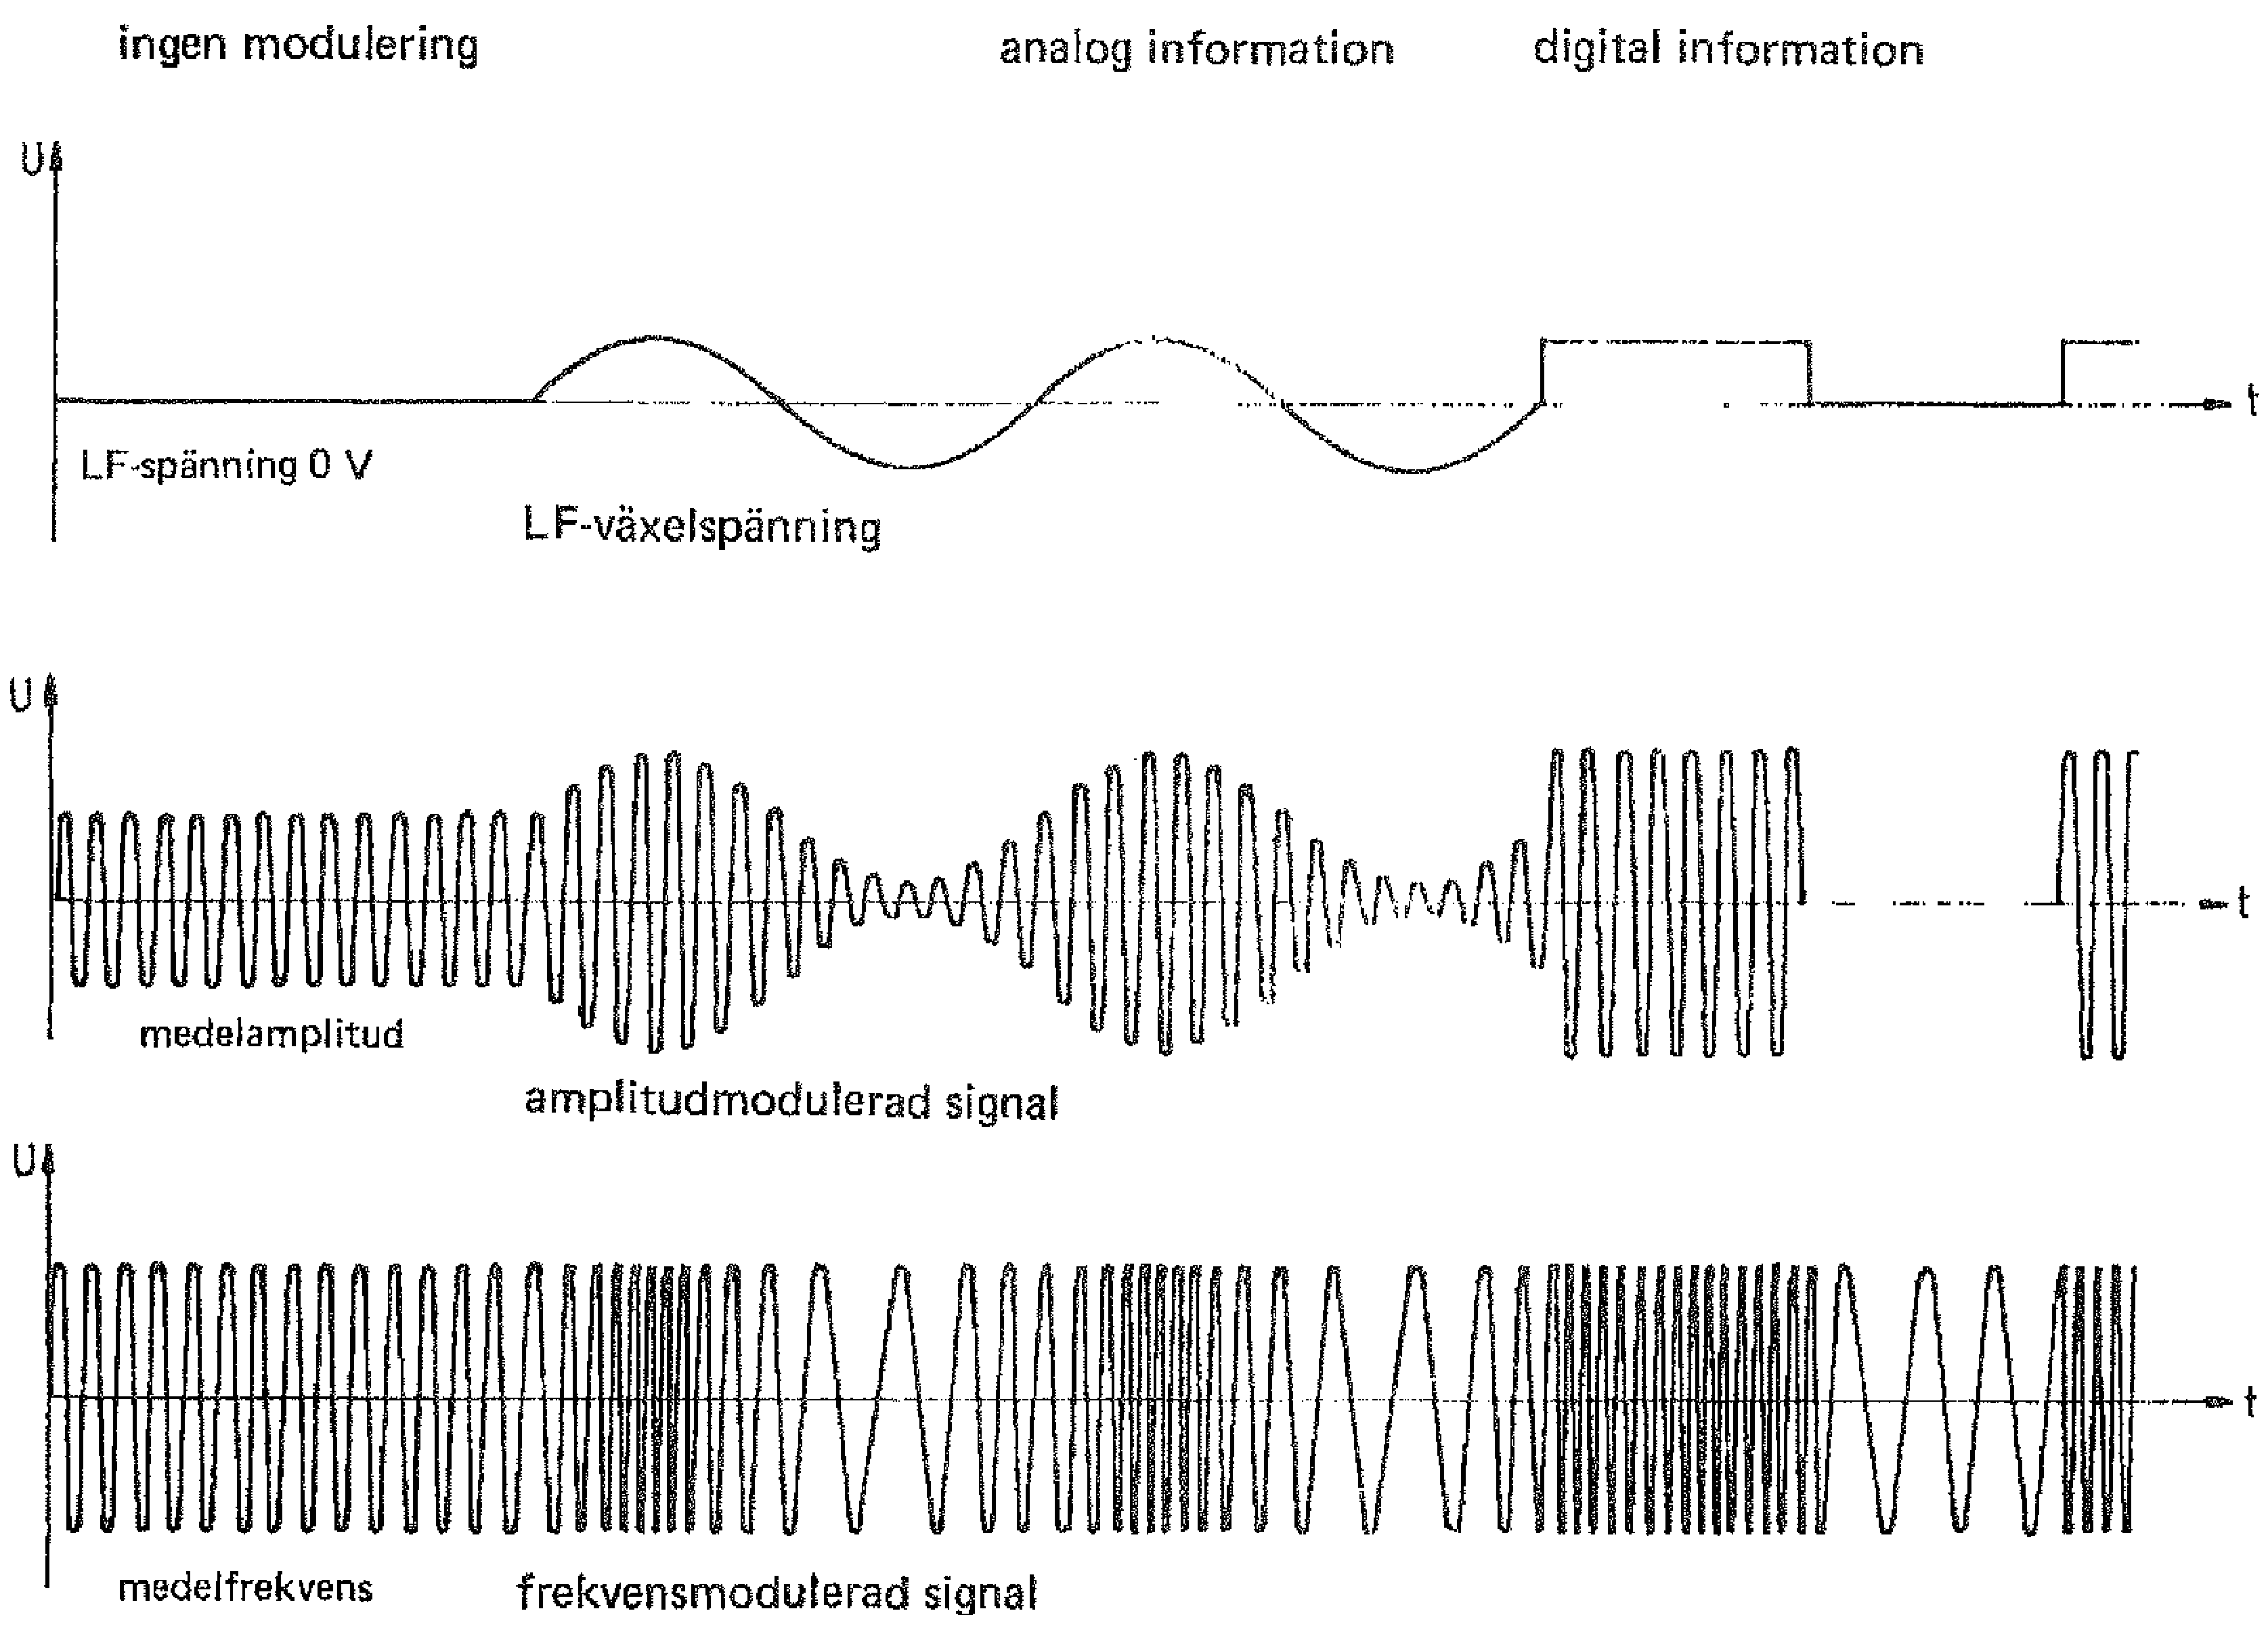
\includegraphics[width=\textwidth]{images/cropped_pdfs/bild_2_1-22.pdf}
\caption{Modulerade signaler}
\label{fig:BildII1-22}
\end{figure}

Bild \ref{fig:BildII1-22}.

En modulerad signal kännetecknas av dess amplitud, frekvens och fasläge.

Vid \emph{amplitudmodulation} påverkas huvudbärvågens amplitud, så att den i
varje tidpunkt motsvarar den modulerande signalens variation.

Vid \emph{frekvensmodulation} påverkas huvudbärvågens frekvens, så att den i
varje tidpunkt motsvarar den modulerande signalens variation.

Vid \emph{fasmodulation}, som är besläktad med frekvensmodulation, påverkas i
stället för frekvensen huvudbärvågens fasläge i förhållande till en
referenssignal, så att fasläget i varje tidpunkt motsvarar den modulerande
signalens variation.

Frekvens- och fasmodulation liknar varandra och kan sammanfattas som
vinkelmodulation, eftersom fasvinkeln mellan bärvågens spänning och ström
varierar i båda fallen.

Vid \emph{pulsmodulation} används pulståg (korta upprepade bärvågspaket); t.ex.
pulsamplitud-, pulslängds-, pulsläges- och pulskodmodulation. Pulskodmodulation
används t.ex. vid samtidig överföring av flera telesamtal på samma linje,
bärvåg etc.

\subsection{Bandbredd vid olika sändningsslag}
\textbf{HAREC a.\ref{HAREC.a.1.8.5}\label{myHAREC.a.1.8.5b}}

Varje radiosändning tar upp plats omkring den nominella bärvågsfrekvensen --
tillsammans \emph{bandbredden}.

Radioamatören måste veta detta ''platsbehov'', främst för att inte sända utanför
de frekvensband som är tilldelade för amatörradioanvändning, men även för att
kunna umgås med annan trafik inom banden.

I alla sändningsslag ökar den använda bandbredden med ökad modulation. Eftersom
största \emph{frekvenseffektivitet} alltid ska eftersträvas så upptar en
sändare med kraftigare modulation än vad som behövs för en överföring, alltid
onödigt frekvensutrymme.

\subsection{Beskrivningskod för sändningsslagen}

Vid 1979 års radioförvaltningskonferens (WARC 79) i Geneve reviderades det
internationella radioreglementet (RR), som i huvudsak trädde i kraft 1982.
Däri ingår bl.a. ett nytt system för klassindelning och beteckning av sätten
att utsända information över radio m.m. Reglementet har reviderats senare, men
i detta stycke gäller det ännu.

Indelningen i sändningsslag behövs för att känneteckna utsändningarna, t.ex. i
frekvenslistor, författningar och föreskrifter. Indelningen är också av stort
värde vid teknisk beskrivning av apparater och system för radiokommunikation.

Emellertid används av många även äldre benämningar, vilka lever kvar i
litteraturen, i märkning av manöverdonen på sändare och mottagare o.s.v.

Dessa äldre benämningar är dock inte entydiga och skapar lätt missförstånd,
varför beskrivningskoden enligt WARC 79 bör användas för tydlighetens skull.

Här följer avkortade koder enligt WARC 79 för några av de sändningsslag, som
amatörer använder mest, samt för jämförelse även de benämningar som fortfarande
används jämsides (se vidare i Appendix E).

\begin{description}
\item[NON] Bärvåg utan modulerande signal. Ingen information.

\item[A1A] Bärvåg med dubbla sidband. En enda kanal med kvantiserad bärvåg.
Ingen modulerande underbärvåg. Telegrafi.

\emph{Även kallat nycklad bärvåg (CW).}

\item[A3E] Linjärt modulerad huvudbärvåg. Dubbla sidband. En enda kanal med
analog information. Telefoni.

\emph{Även kallat amplitudmodulation (AM).}

\item[J3E] Linjärt modulerad huvudbärvåg. Ett sidband med undertryckt bärvåg.
En enda kanal med analog information. Telefoni.

\emph{Även kallat enkelt sidband (Single Side Band -- SSB).}

\item[F3E] Vinkelmodulerad bärvåg. Frekvensmodulering. En enda kanal med analog
information. Telefoni.

\emph{Även kallat frekvensmodulering (FM).}

\item[G3E] Vinkelmodulerad bärvåg. Fasmodulering. En enda kanal med analog
information. Telefoni.

\emph{Även kallat fasmodulering (PM).}
\end{description}

Såväl A1A, A3E som J3E är sändningsslag där amplituden moduleras. Därför är
termen \emph{amplitudmodulation} inte tillräcklig för att beskriva flera
likartade sändningsslag.

\subsection{Modulerande signaler}
\textbf{HAREC a.\ref{HAREC.a.1.7.1}\label{myHAREC.a.1.7.1}}
\index{modulerande signaler}

\subsubsection{Basband}
\index{basband}

Basband är ett frekvensområde för en modulerande signal. Det finns ett basband
för alla slags modulerande signaler, vare sig de är analoga eller digitala. Det
kan finnas mer än ett basband i en komplett modulationsprocess. Till exempel är
en nycklad ton, som går till sändaren genom mikrofoningången, dess analoga
basband medan nycklingspulserna till tongeneratorn är dess digitala basband.

\begin{figure}
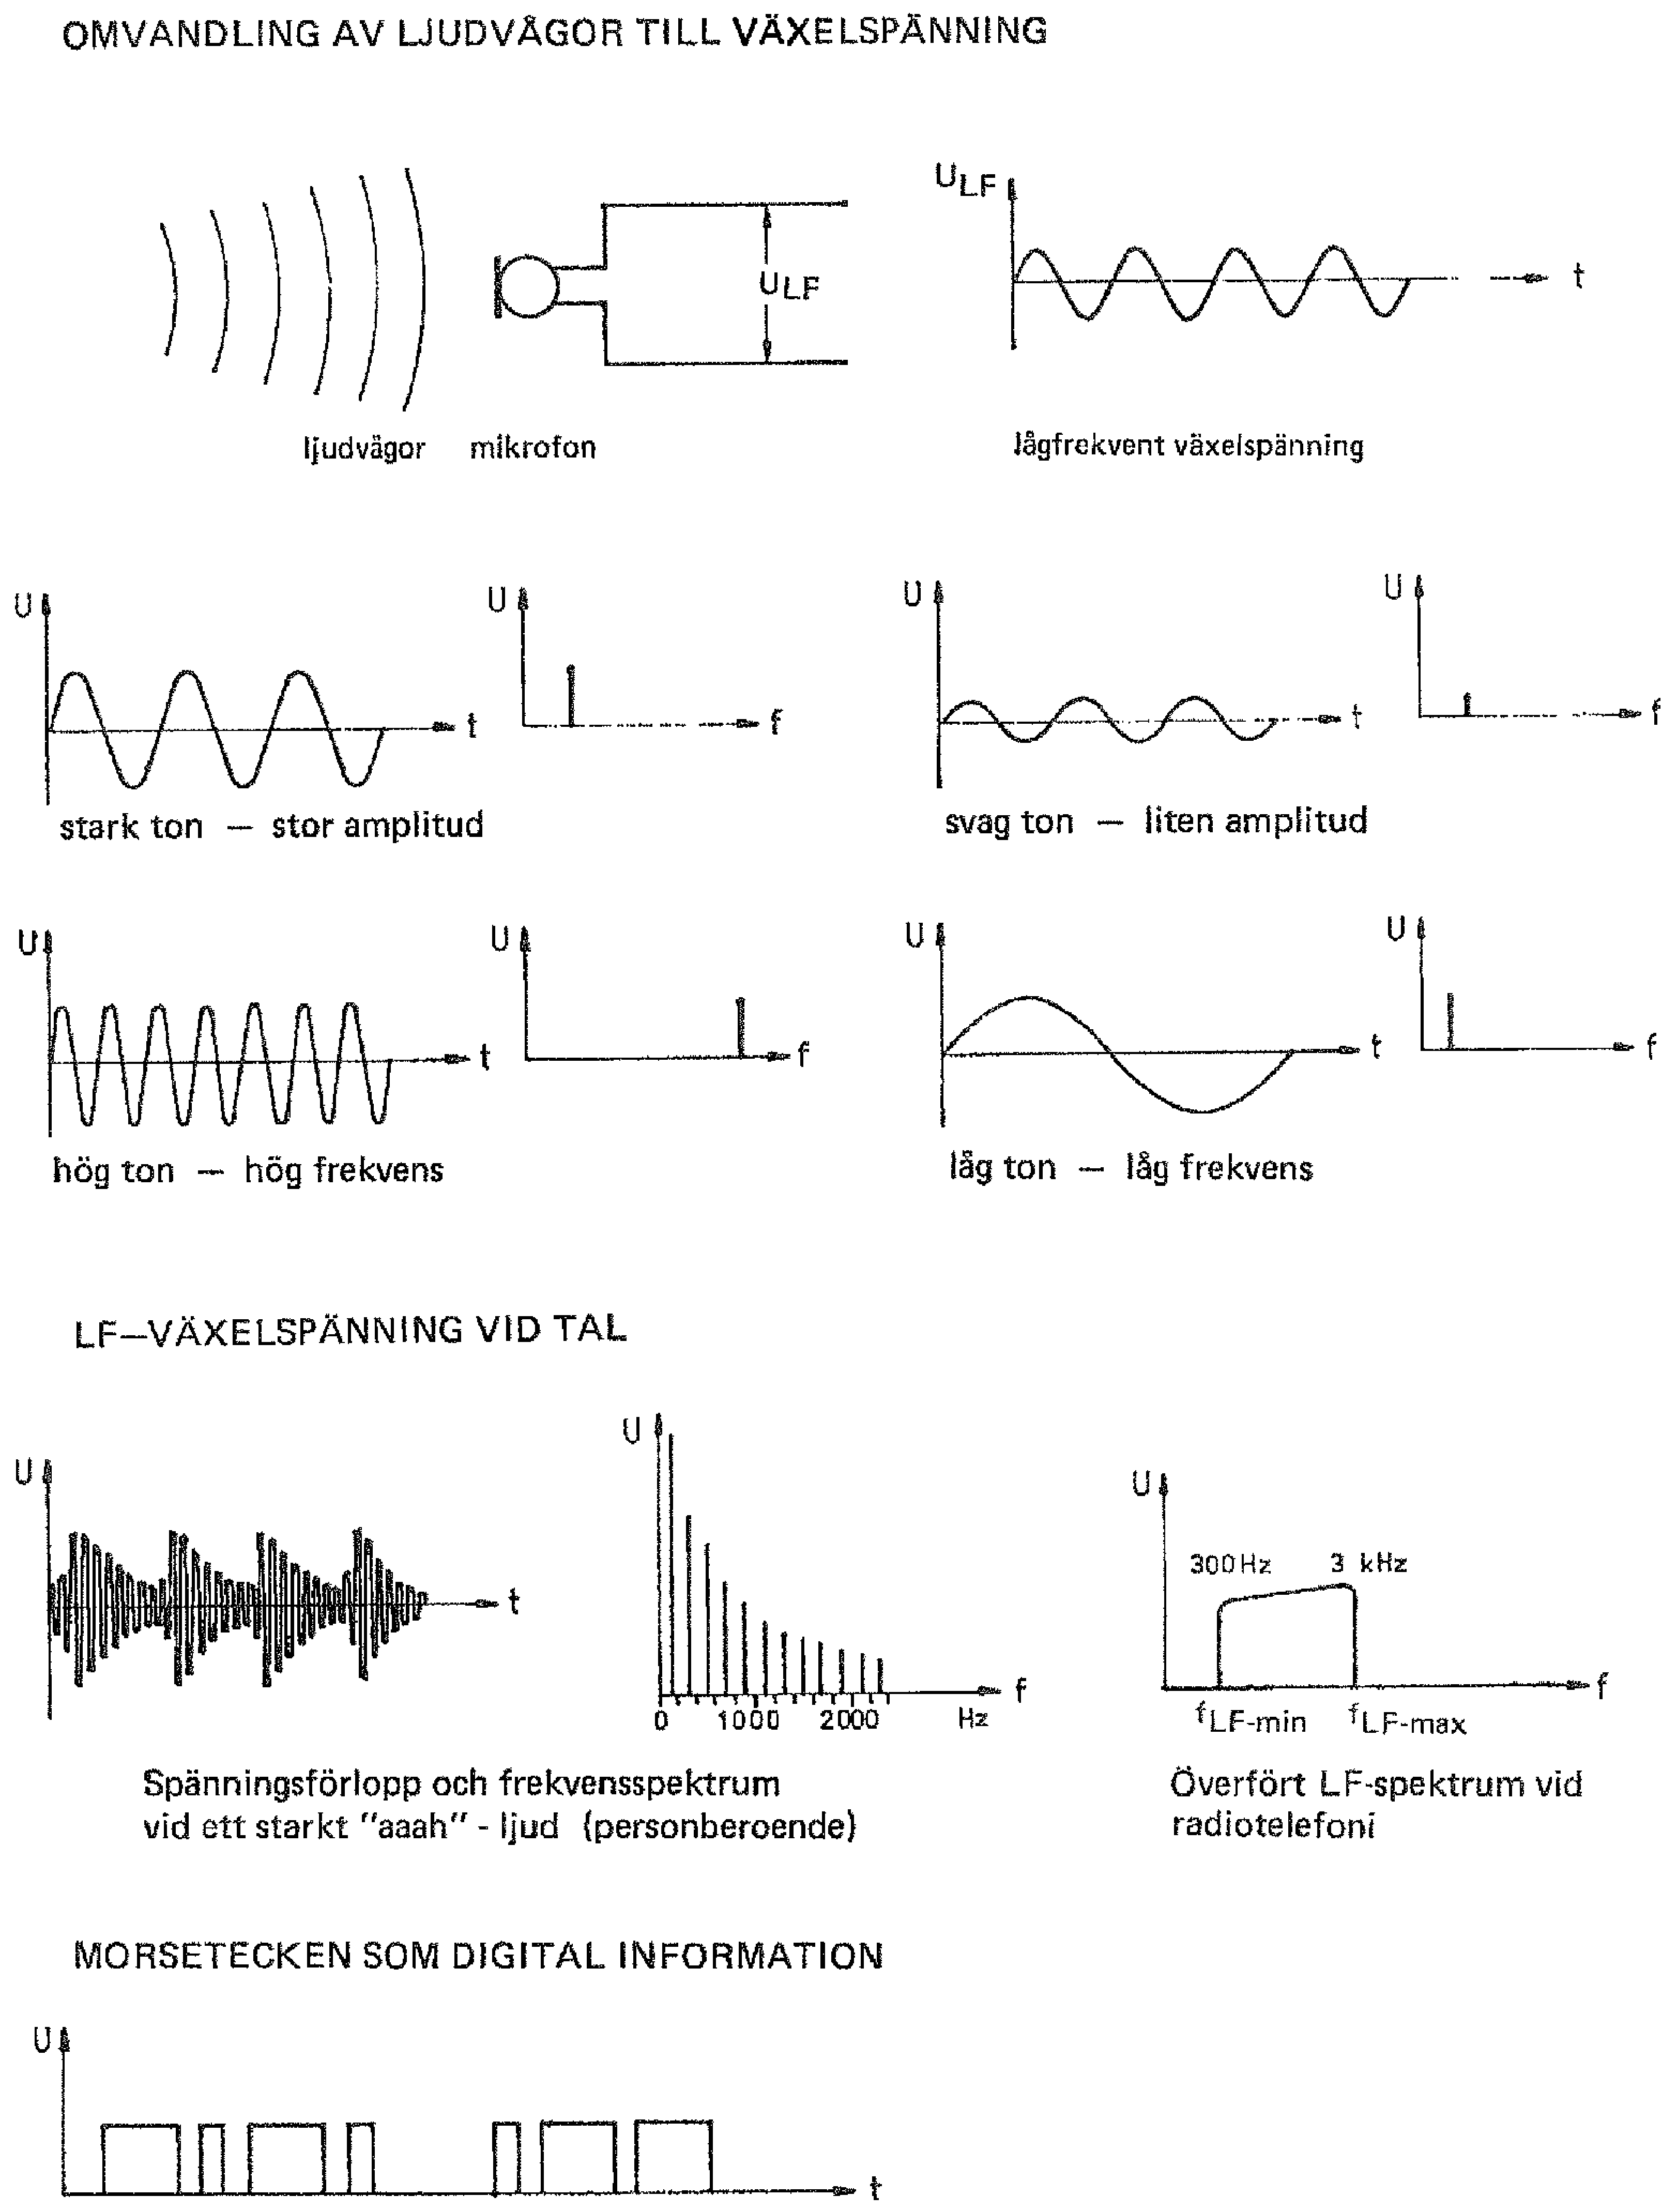
\includegraphics[width=\textwidth]{images/cropped_pdfs/bild_2_1-23.pdf}
\caption{Modulerande signaler}
\label{fig:BildII1-23}
\end{figure}

Bild \ref{fig:BildII1-23}.

Ett vanligt sätt att överföra information över radio är med telefoni, d.v.s.
tal.

Frekvensområdet 300--3000~Hz räcker för god förståelighet av tal. Dels är örat
känsligast inom det området och dels finns där den mesta energin i talet.

Mikrofonen tar upp de lufttrycksvariationer, som uppstår när man talar, och
omvandlar dem till elektriska svängningar. Svängningarna varierar mellan
positiva och negativa spänningsvärden.

\subsubsection{Försök}

\begin{enumerate}
\item Anslut en mikrofon till ett oscilloskop och studera spänningsförloppen
för olika slags ljud, toner, tal osv. som funktion av tiden. På bilden är
dessa svängningar mycket förenklade, t.ex. sinusformade.

\item Anslut en högtalare och ett oscilloskop till en LF-generator, vars
frekvens och amplitud kan ändras. Lyssna på ljud med låg och hög frekvens samt
på svaga och starka ljud. En baston har låg frekvens och en diskantton har hög
frekvens. En svag ton har liten amplitud och en stark ton har stor amplitud.
\end{enumerate}

\subsection{Sändningsslaget A3E (även kallat AM)}
\textbf{HAREC a.\ref{HAREC.a.1.8.2}, a.\ref{HAREC.a.1.8.6b}, a.\ref{HAREC.a.1.8.7b}\label{myHAREC.a.1.8.2}\label{myHAREC.a.1.8.6b}\label{myHAREC.a.1.8.7b}}
\index{amplitudmodulation}
\index{A3E}
\index{AM}

\begin{figure}
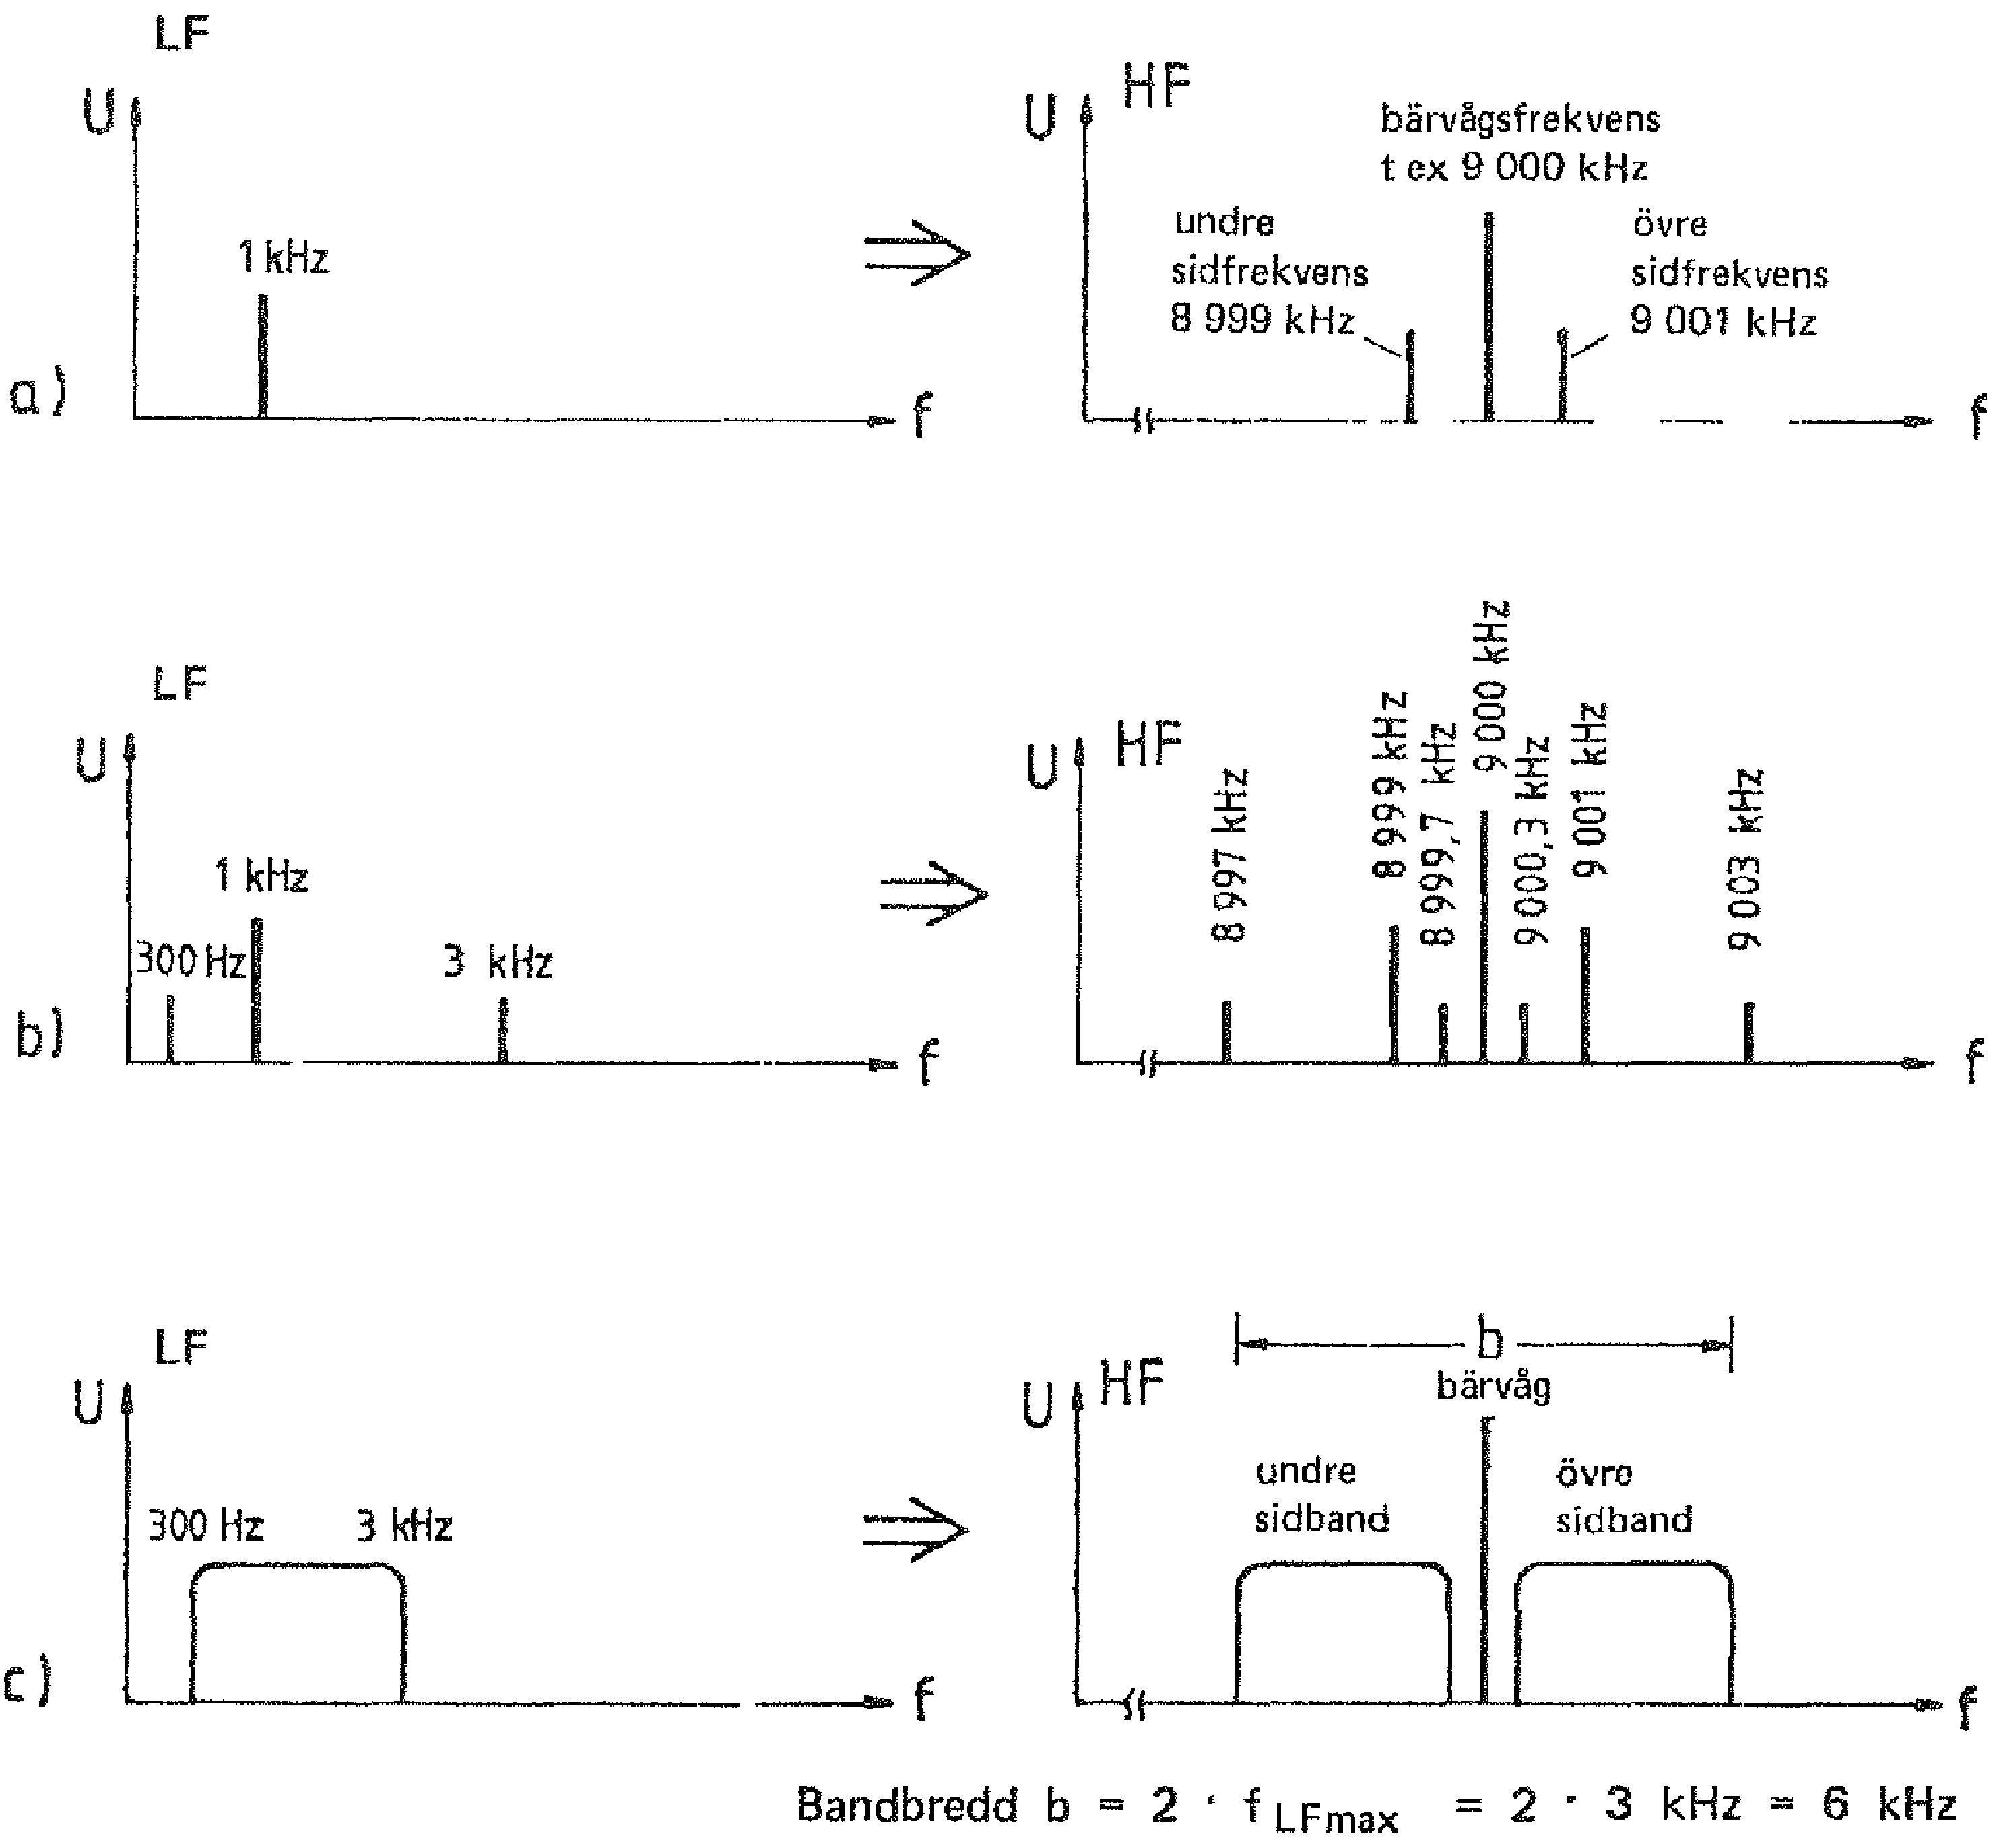
\includegraphics[width=\textwidth]{images/cropped_pdfs/bild_2_1-24.pdf}
\caption{Sidband vid A3E-modulation}
\label{fig:BildII1-24}
\end{figure}

Bild \ref{fig:BildII1-24}.

Bilden visar frekvensspektrum av en signal vid amplitudmodulation med

\begin{enumerate}[label=\alph*.,noitemsep]
\item en sinuston,
\item en blandning av tre sinustoner,
\item ett frekvensspektrum.
\end{enumerate}

\subsubsection{Försök}

Modulera en A3E-sändare med en 3~kHz signal. Med en mottagare utrustad med ett
smalt filter för telegrafi, kan man urskilja och påvisa bärvågen och de båda
sidbanden.

\subsubsection{A3E-modulation med en ton}

\begin{figure}
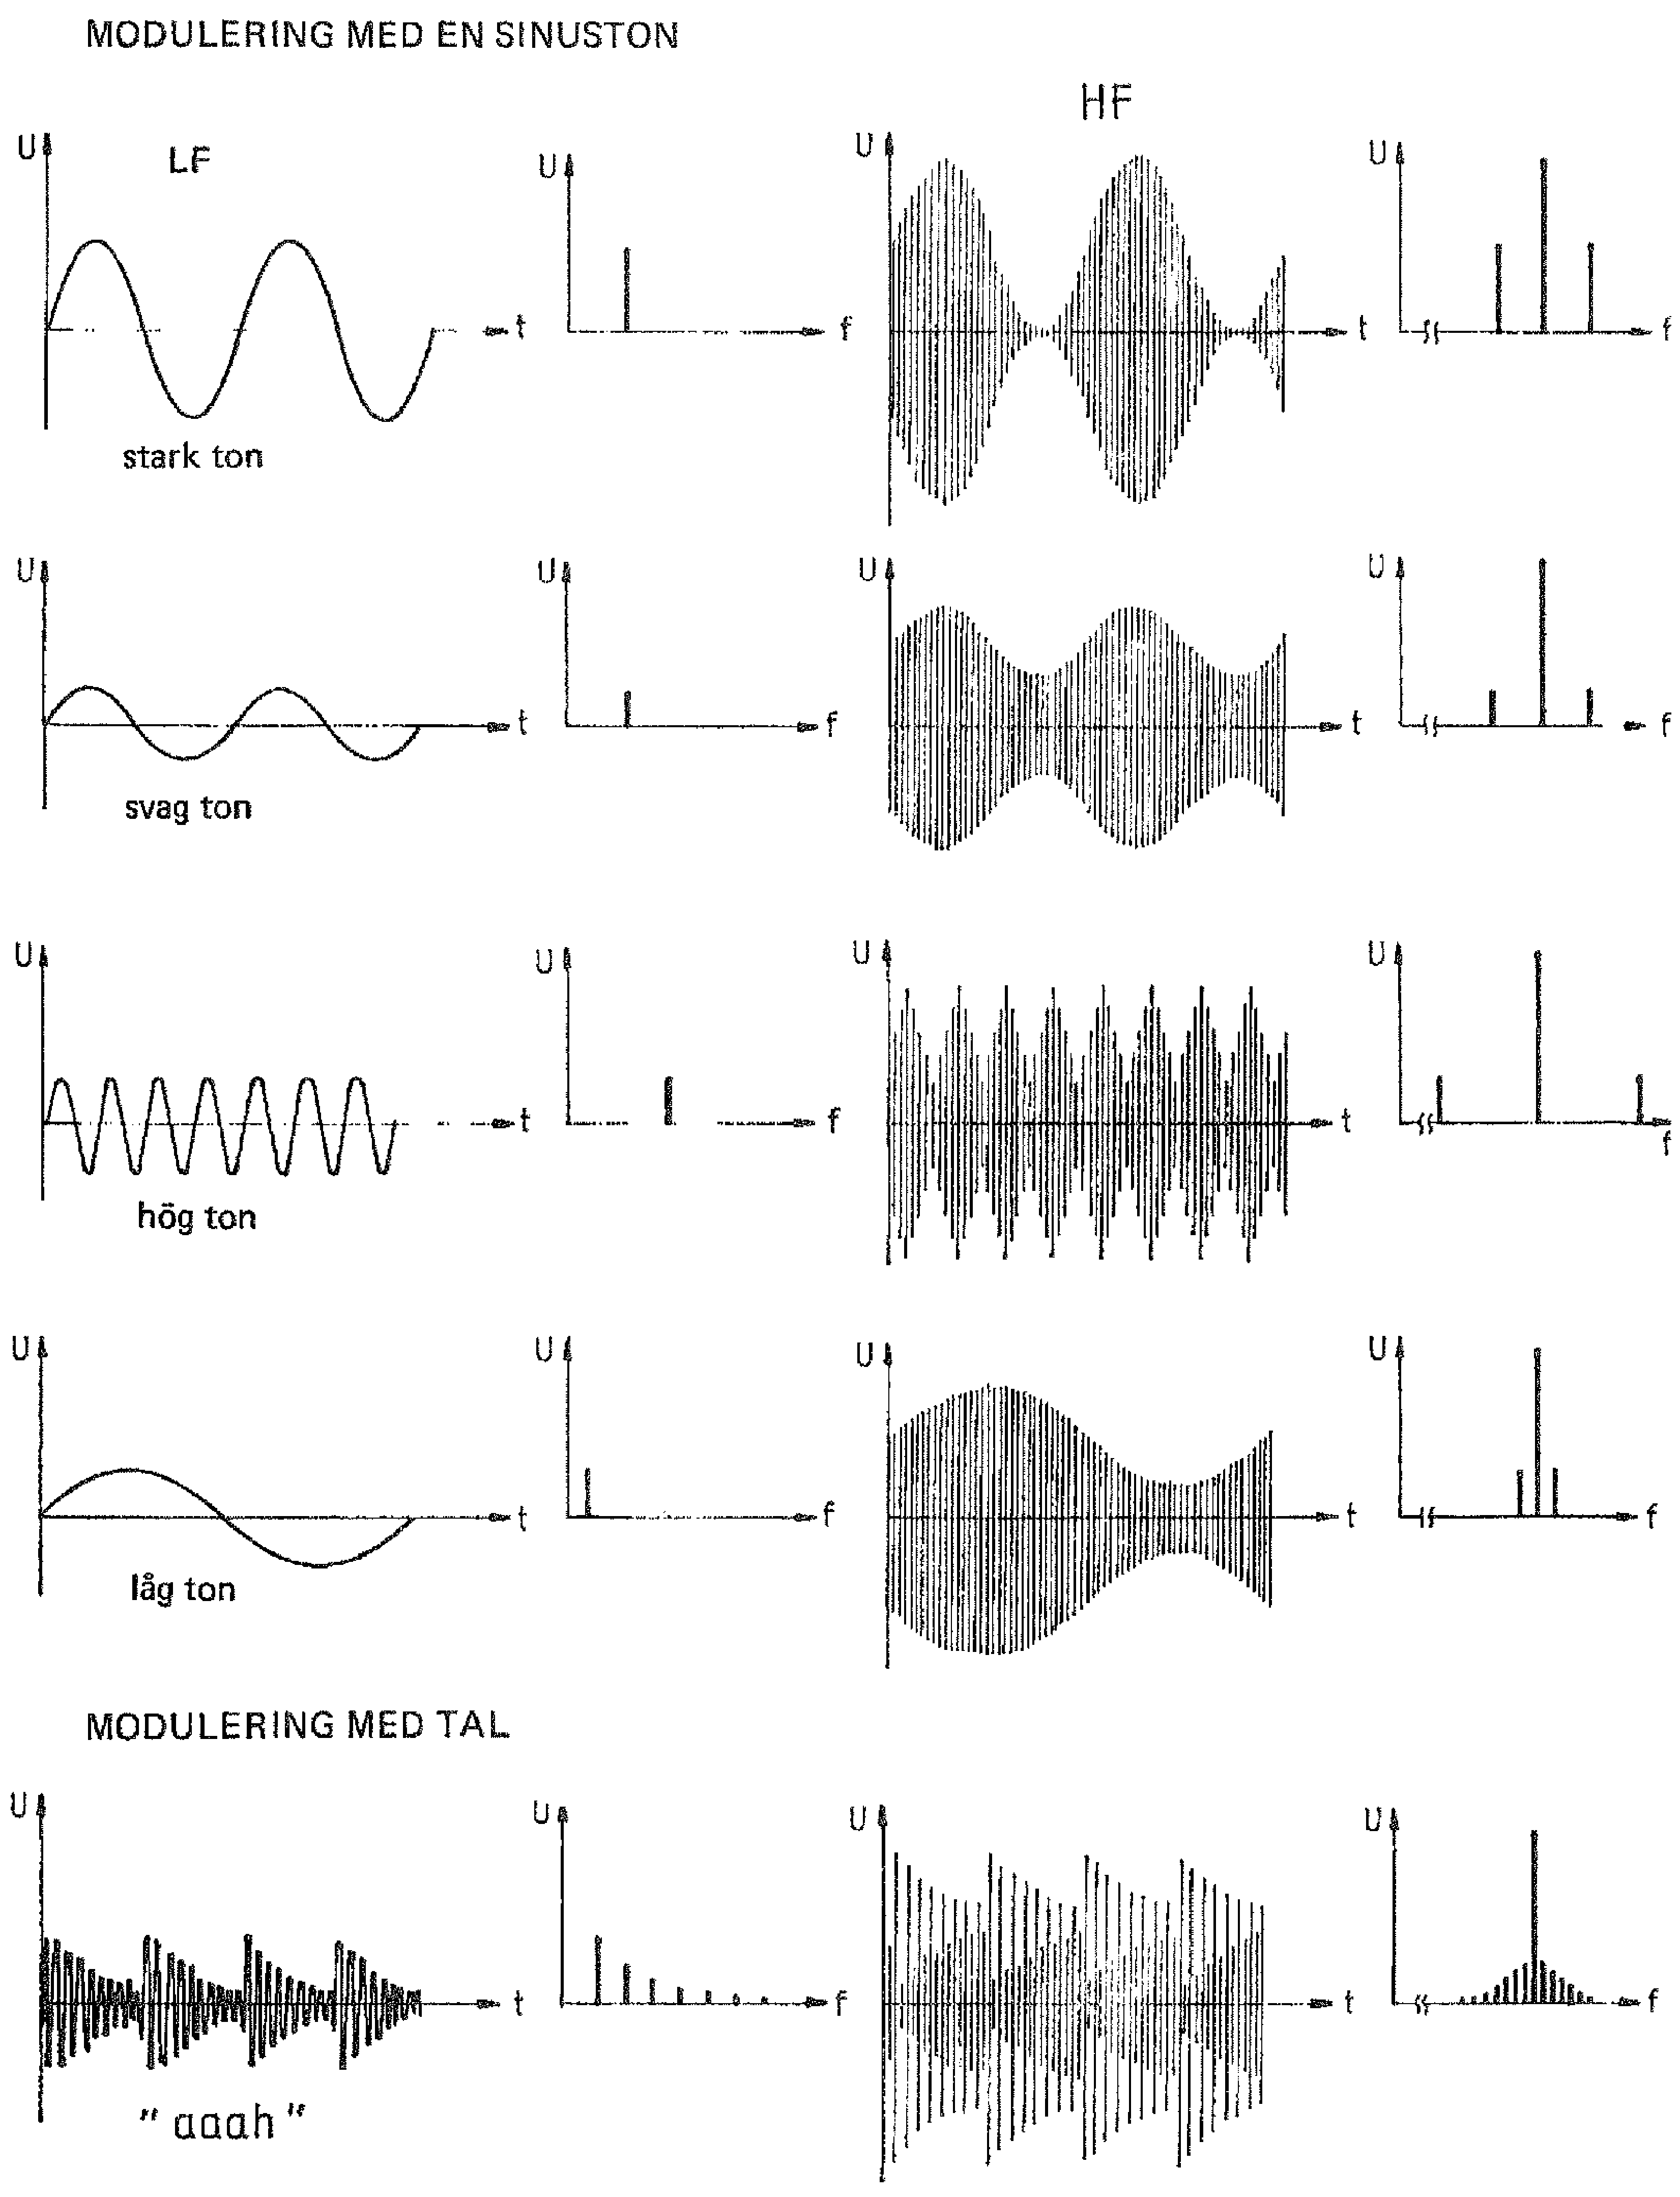
\includegraphics[width=\textwidth]{images/cropped_pdfs/bild_2_1-25.pdf}
\caption{A3E-modulation med toner med olika styrka och frekvens}
\label{fig:BildII1-25}
\end{figure}

Bild \ref{fig:BildII1-25}.

En omodulerad bärvåg har konstant amplitud. En amplitudmodulerad signal är i
grunden resultatet av svävning mellan frekvenser eller av icke linjär blandning
av frekvenser. När bärvåg och basband blandas, så är särskilt tre
blandningsprodukter av intresse.

Dessa är

\begin{enumerate}[label=-,noitemsep]
\item bärvågen,
\item det lägre sidbandet (förkortat LSB) och
\item det övre sidbandet (förkortat USB).
\end{enumerate}

AM-signalen består således inte bara av bärvågsfrekvensen \(f_{HF}\) utan även
av övre och nedre sidofrekvenser, vilka är summan och skillnaden av
bärvågsfrekvensen \(f_{HF}\) och den modulerande frekvensen \(f_{LF}\).
Alltså \(f_{HF} + f_{LF}\) (övre sidofrekvens) och skillnadsfrekvensen
\(f_{HF} - f_{LF}\) (undre sidofrekvens).

Eftersom tal inte bara omfattar en enda frekvens utan ett helt frekvensspektrum
(ca 0,3--3~kHz), så uppstår inte bara två sidofrekvenser utan två sidband, det
lägre sidbandet (LSB, Lower Side Band) och det övre (USB, Upper Side Band).

LF-signalens frekvens bestämmer sidofrekvensens avstånd från bärvågen.
Bandbredden på en amplitudmodulerad signal med full bärvåg och två sidband är
dubbelt så stor som den högsta modulerande LF-frekvensen:

\(b= 2 \cdot f_{LFmax}\)

Om de modulerande LF-frekvenserna är mellan 0,3 och 3~kHz, så blir sändningens
totala bandbredd 6~kHz.

LF-signalernas amplitud påverkar sidbandens och sidofrekvensernas amplitud. Vid
maximal modulation (100~\% modulationsgrad) varierar signalamplituden mellan
noll och dubbla värdet av det för en omodulerad bärvåg.

Som mest kan vardera sidbandet överföra en fjärdedel så mycket effekt som
bärvågen, d.v.s. en sjättedel av den totalt utsända effekten. Då avger sändaren
dubbelt så stor medeleffekt som utan modulation. Toppeffekten (PEP,
Peak Envelope Power) är till och med fyra gånger så stor.

Slutförstärkaren och kraftförsörjningen måste dimensioneras för toppeffekten vid
full modulation eller att modulationsgraden anpassas så att överbelastning inte
sker.

\subsubsection{Fördelar med A3E-modulation}

En A3E-sändare är enkel jämfört med en J3E-sändare, vilken har en mer
komplicerad signalbehandling.

\subsubsection{Nackdelar med A3E-modulation}

Eftersom samma information finns i båda sidbanden och ingen finns i bärvågen,
så sänds effekten i bärvågen och ett av sidbanden ut till ingen nytta. I
talpauser sänds endast bärvågseffekten och till ingen nytta. Även
frekvensutrymme slösas bort. Då en annan, alltför närliggande sändares bärvåg
blandas med den egna, så alstras interferenstoner i mottagarna.

\subsection{Sändningsslaget A1A (även kallat CW)}
\textbf{HAREC a.\ref{HAREC.a.1.8.1}, a.\ref{HAREC.a.1.8.6a}, a.\ref{HAREC.a.1.8.7a}\label{myHAREC.a.1.8.1}\label{myHAREC.a.1.8.6a}\label{myHAREC.a.1.8.7a}}
\index{A1A}
\index{CW}

\begin{figure}
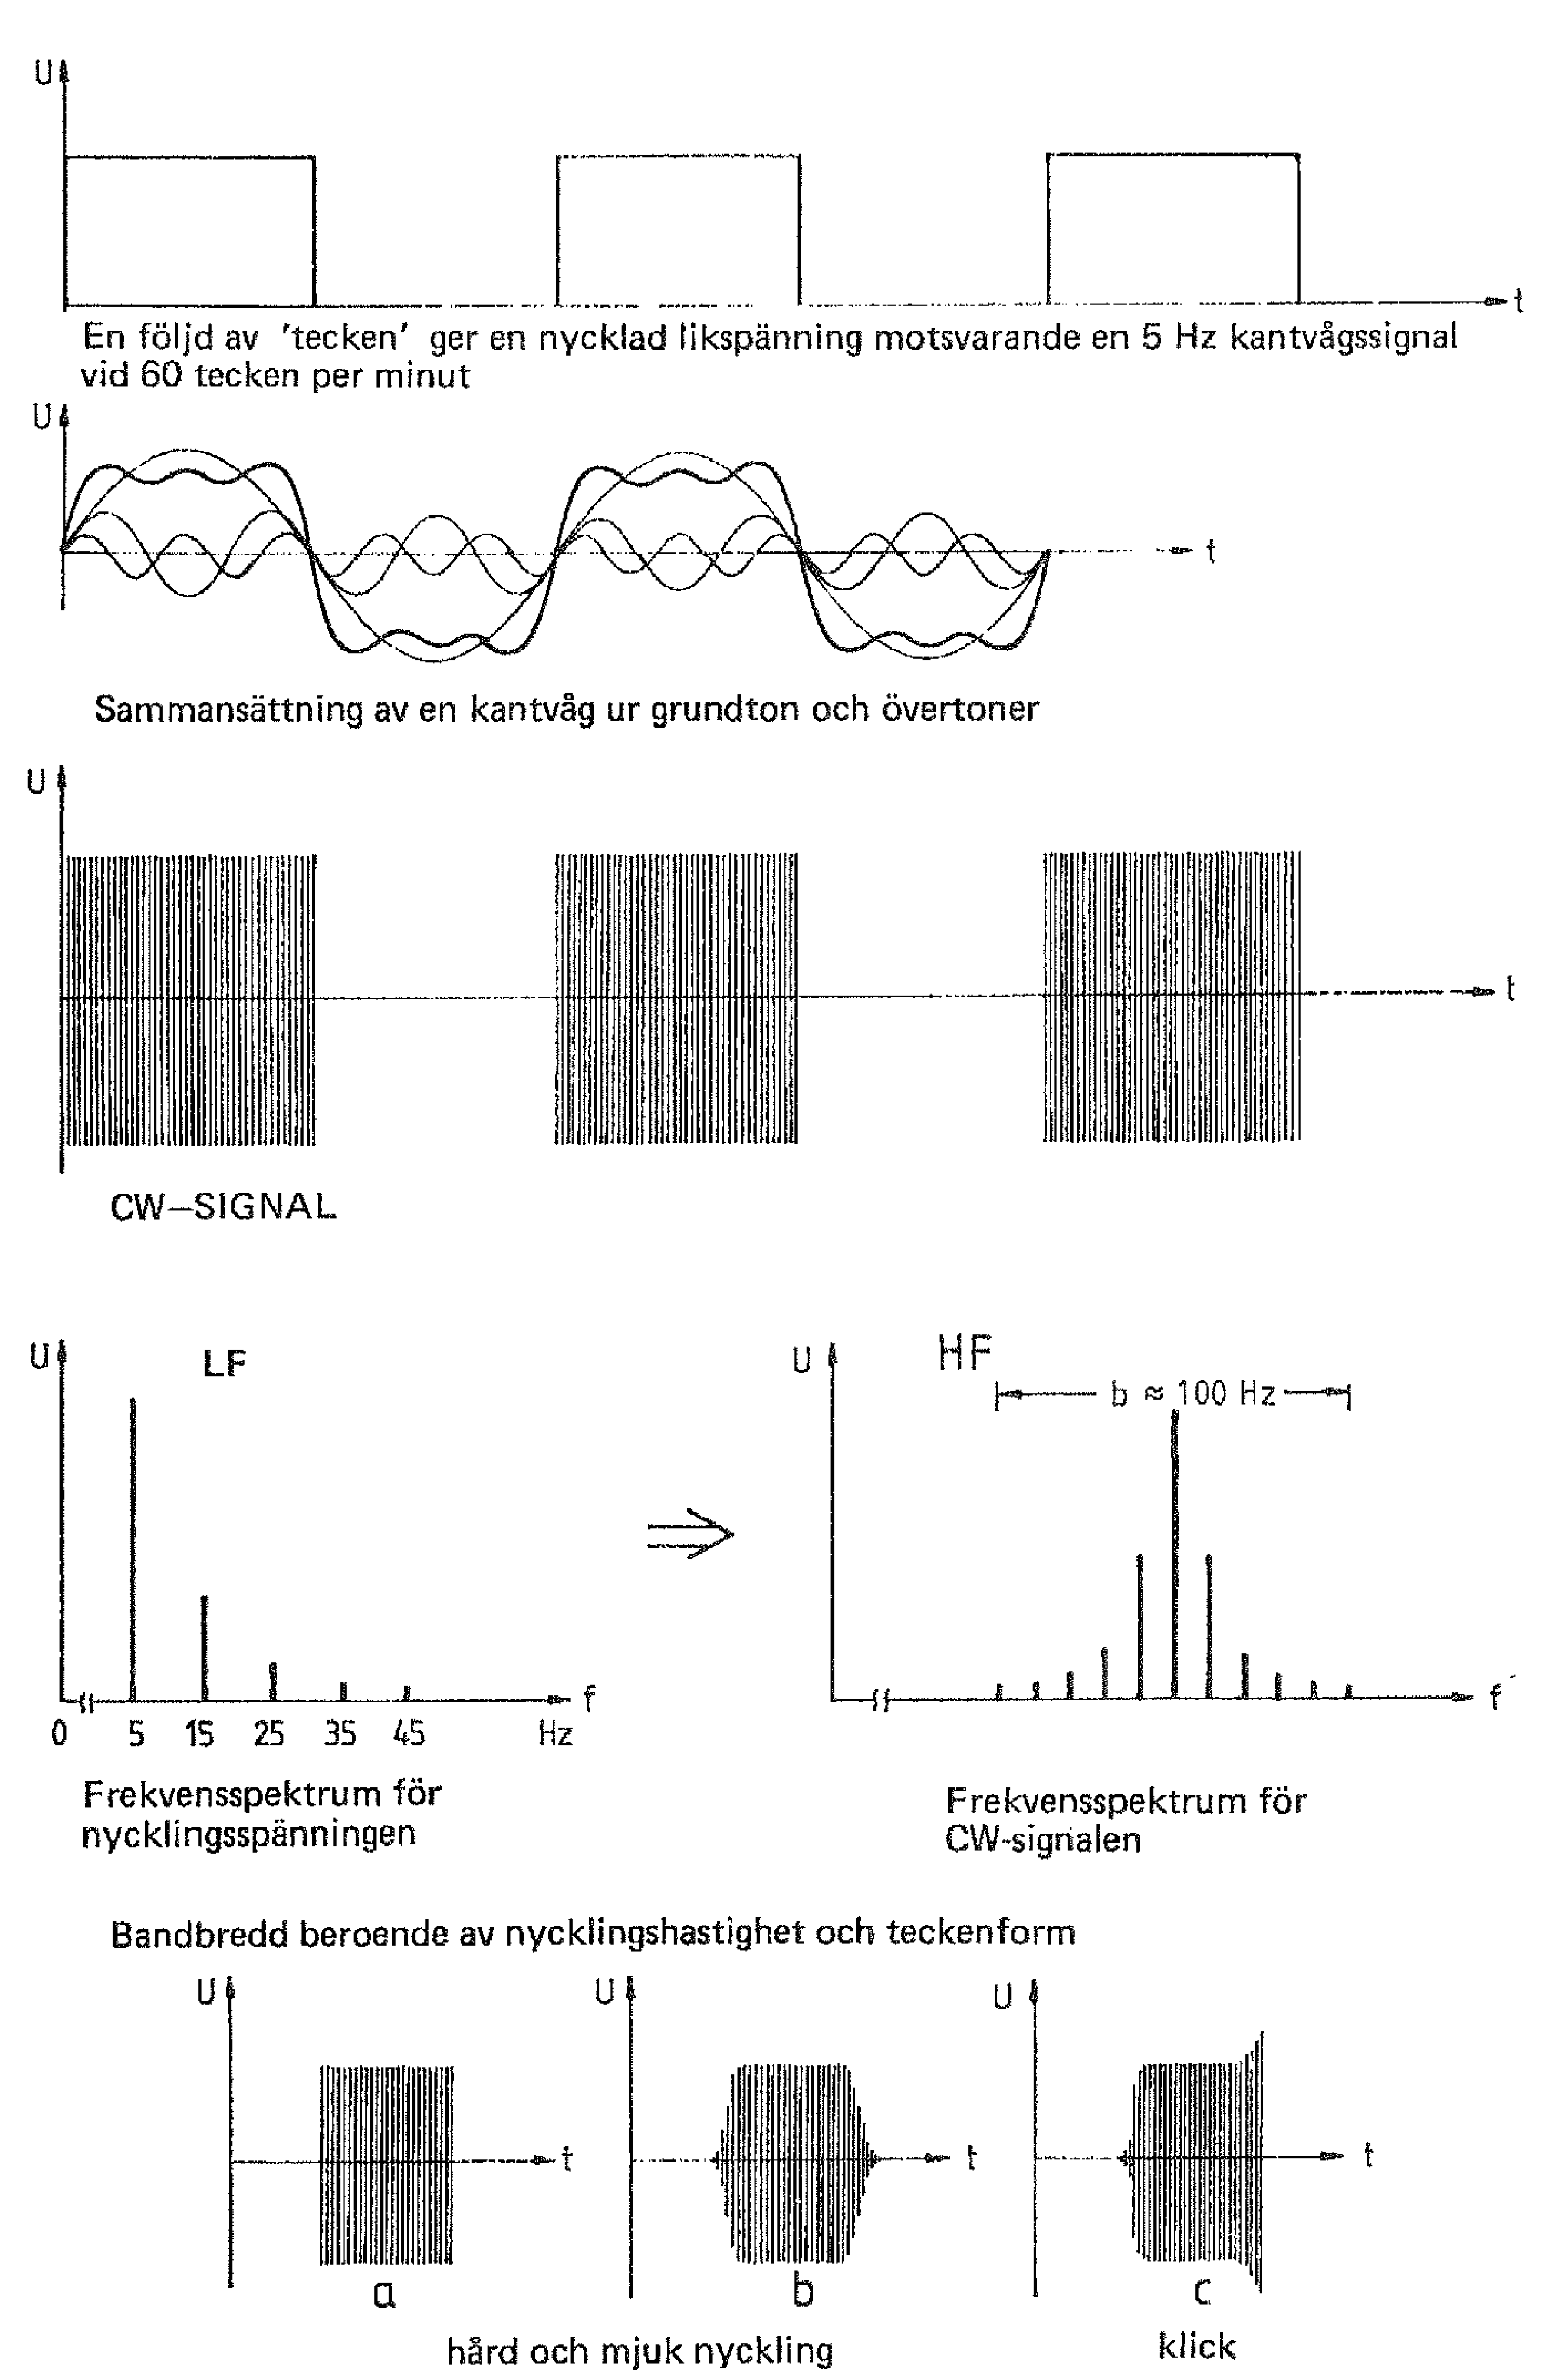
\includegraphics[width=\textwidth]{images/cropped_pdfs/bild_2_1-26.pdf}
\caption{Amplitudmodulation med morsetecken}
\label{fig:BildII1-26}
\end{figure}

Bild \ref{fig:BildII1-26}.

Man kan överföra meddelanden med morsetelegrafi på olika sätt. Det enklaste
sättet är att koppla in och ur sändarens bärvåg i takt med teckendelarna i
morsetecknen. Man kan kalla det för bärvågstelegrafi. Förfarandet kallas sedan
mycket länge även för CW (continous waves), vilket egentligen anger att
bärvågen svänger med konstant amplitud, om man bortser från att den nycklas.
Detta i motsats till de dämpade bärvågssvängningar som var fallet i sedan
mycket länge förbjudna s.k. gnistsändare.

Fastän en sändare ''moduleras utan ton'', har den en viss bandbredd. Det beror på
att den takt, som sändaren nycklas med, egentligen är en ton -- låt vara med låg
frekvens. Antag att sändaren nycklas med en serie korta morsetecken. Vid
telegraferingshastigheten 60 tecken/minut alstrar bärvågspulserna en kantvåg
med frekvensen 5~Hz. Som tidigare beskrivits, består en sådan kantvåg av summan
av sinussignaler med frekvenserna 5~Hz, 15~Hz, 25~Hz, 35~Hz o.s.v.

Det innebär att det uppstår sidofrekvenser över och under bärvågens frekvens och
med ett avstånd till bärvågen av 5~Hz, 15~Hz, 25~Hz, 35~Hz o.s.v ..
Telegrafisändaren har alltså liksom vid A3E en bandbredd, som dels står i
förhållande till nycklingshastigheten och dels till ''kantigheten'' på tecknen,
vilket bestämmer övertonshalten i bärvågen. Vid s.k. mjuk nyckling kan den 9:e
övertonen antas vara den högsta som uppfattas av en motstation. Med en
nycklingsfrekvens av 5~Hz blir bandbredden inte större än
\(2 \cdot 10 \cdot 5 = 100\ Hz\).

En hård (kantig) och snabb teckengivning ökar bandbredden och kan resultera i
att s.k. nycklingsknäppar kan uppfattas långt vid sidan om sändningsfrekvensen.
Ju hårdare nycklingen är, desto längre bort från bärvågsfrekvensen hörs
nycklingsknäpparna. Detta stör andra stationer.

Kännetecken för sändningsslaget A1A, telegrafi genom nycklad bärvåg:

Mycket liten bandbredd, extremt gott utnyttjande av sändareffekten, stor
överföringssäkerhet, lång räckvidd, enkla sändare.

\subsection{Sändningsslaget J3E (även kallat SSB)}
\textbf{HAREC a.\ref{HAREC.a.1.8.3c}, a.\ref{HAREC.a.1.8.6c}, a.\ref{HAREC.a.1.8.7c}\label{myHAREC.a.1.8.3c}\label{myHAREC.a.1.8.6c}\label{myHAREC.a.1.8.7c}}
\index{single side band}
\index{J3E}
\index{SSB}

\subsubsection{Princip}

Som sagts är det onödigt sända ut två sidband, eftersom båda innehåller samma
information.

Signaler med endast ett sidband och undertryckt bärvåg kan alstras på flera
sätt. Numera är den s.k. filtermetoden i särklass vanligast och den enda som
behandlas här.

\begin{figure}
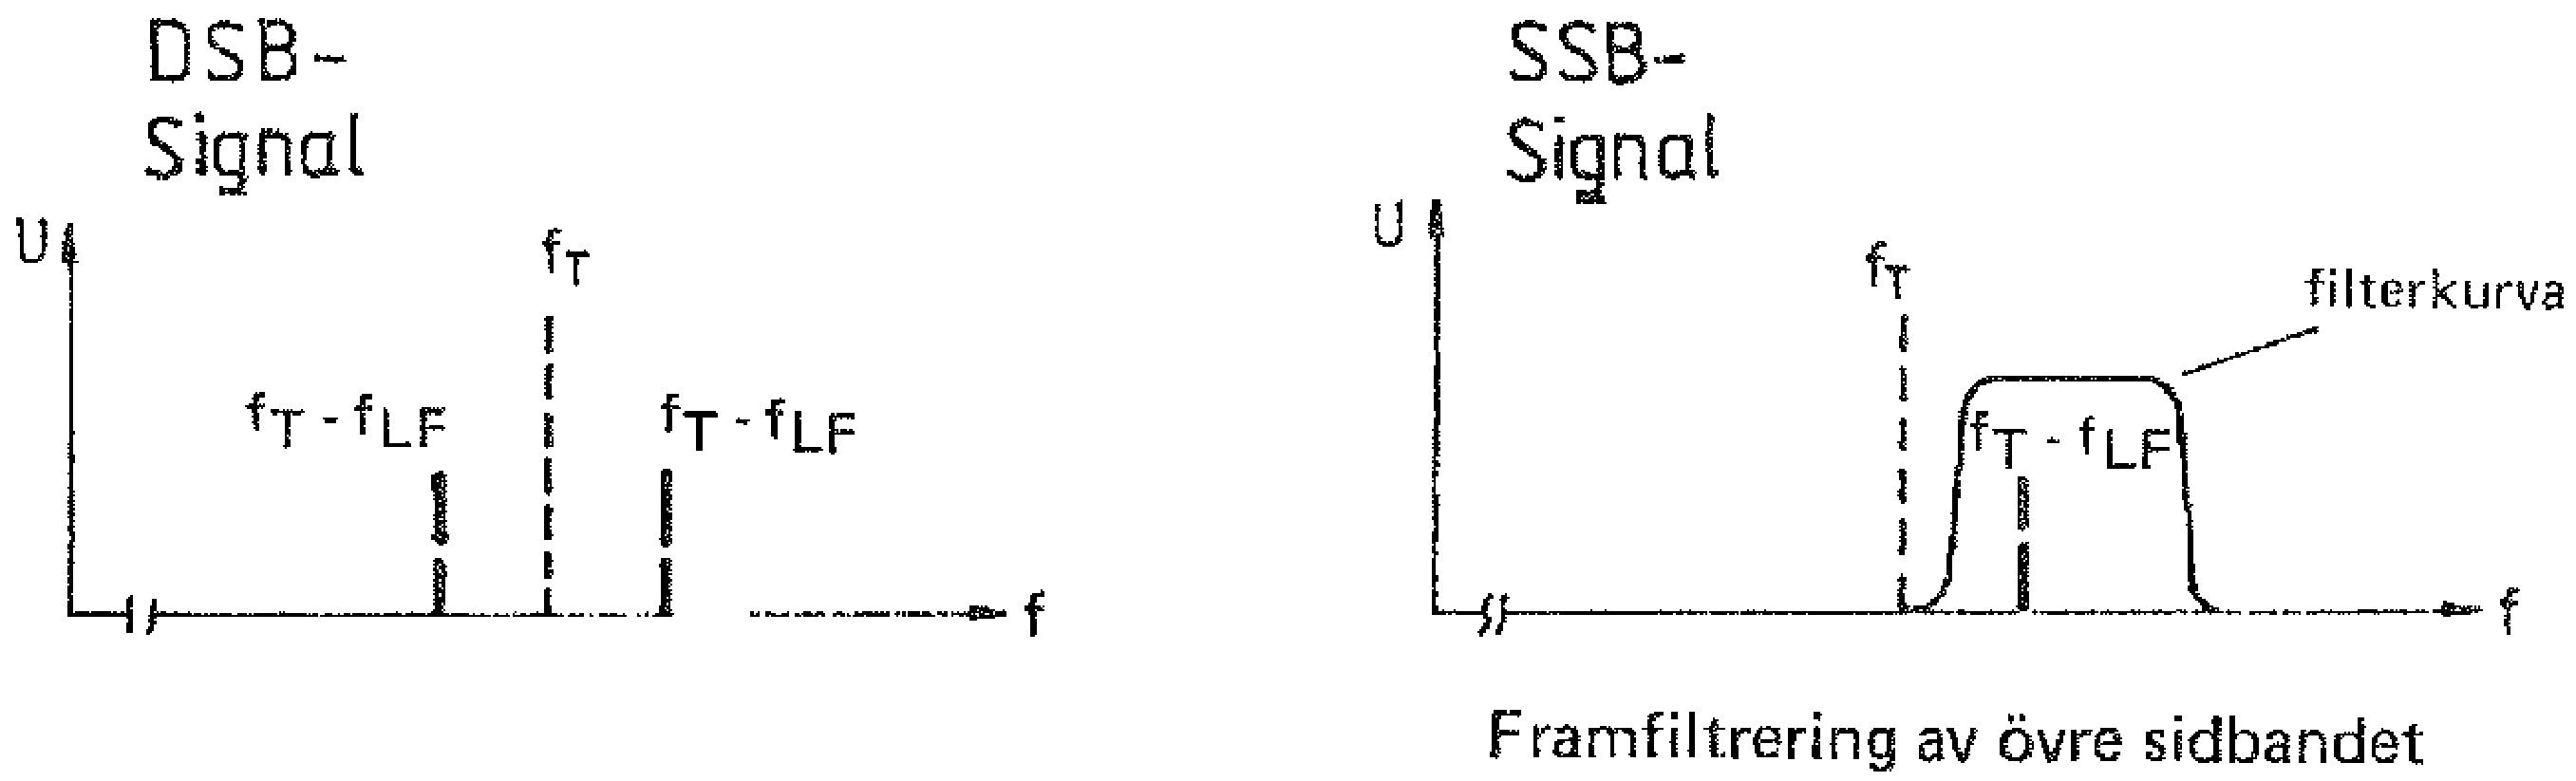
\includegraphics[width=\textwidth]{images/cropped_pdfs/bild_2_1-27.pdf}
\caption{Sidband vid DSB}
\label{fig:BildII1-27}
\end{figure}

Bild \ref{fig:BildII1-27}.

Med filtermetoden blandas HF- och LF-signalerna i en speciell blandare. Där
undertrycks båda dessa signaler medan blandningsprodukterna med deras summa-
och skillnadsfrekvenser blir kvar, d.v.s. det övre och nedre sidbandet.

Utsignalen från blandaren benämns DSB-signal (Double Side Band). Till skillnad
från i A3E-signalen saknas dock bärvågen i DSB-signalen. För att även
undertrycka det ena sidbandet före sändningen, så följs blandaren av ett
bandpassfilter med bandbredd och frekvensläge för avsett sidband.

Den signal som sänds ut innehåller därför endast ett sidband (Single Side Band).

\paragraph{Exempel}

\begin{figure}
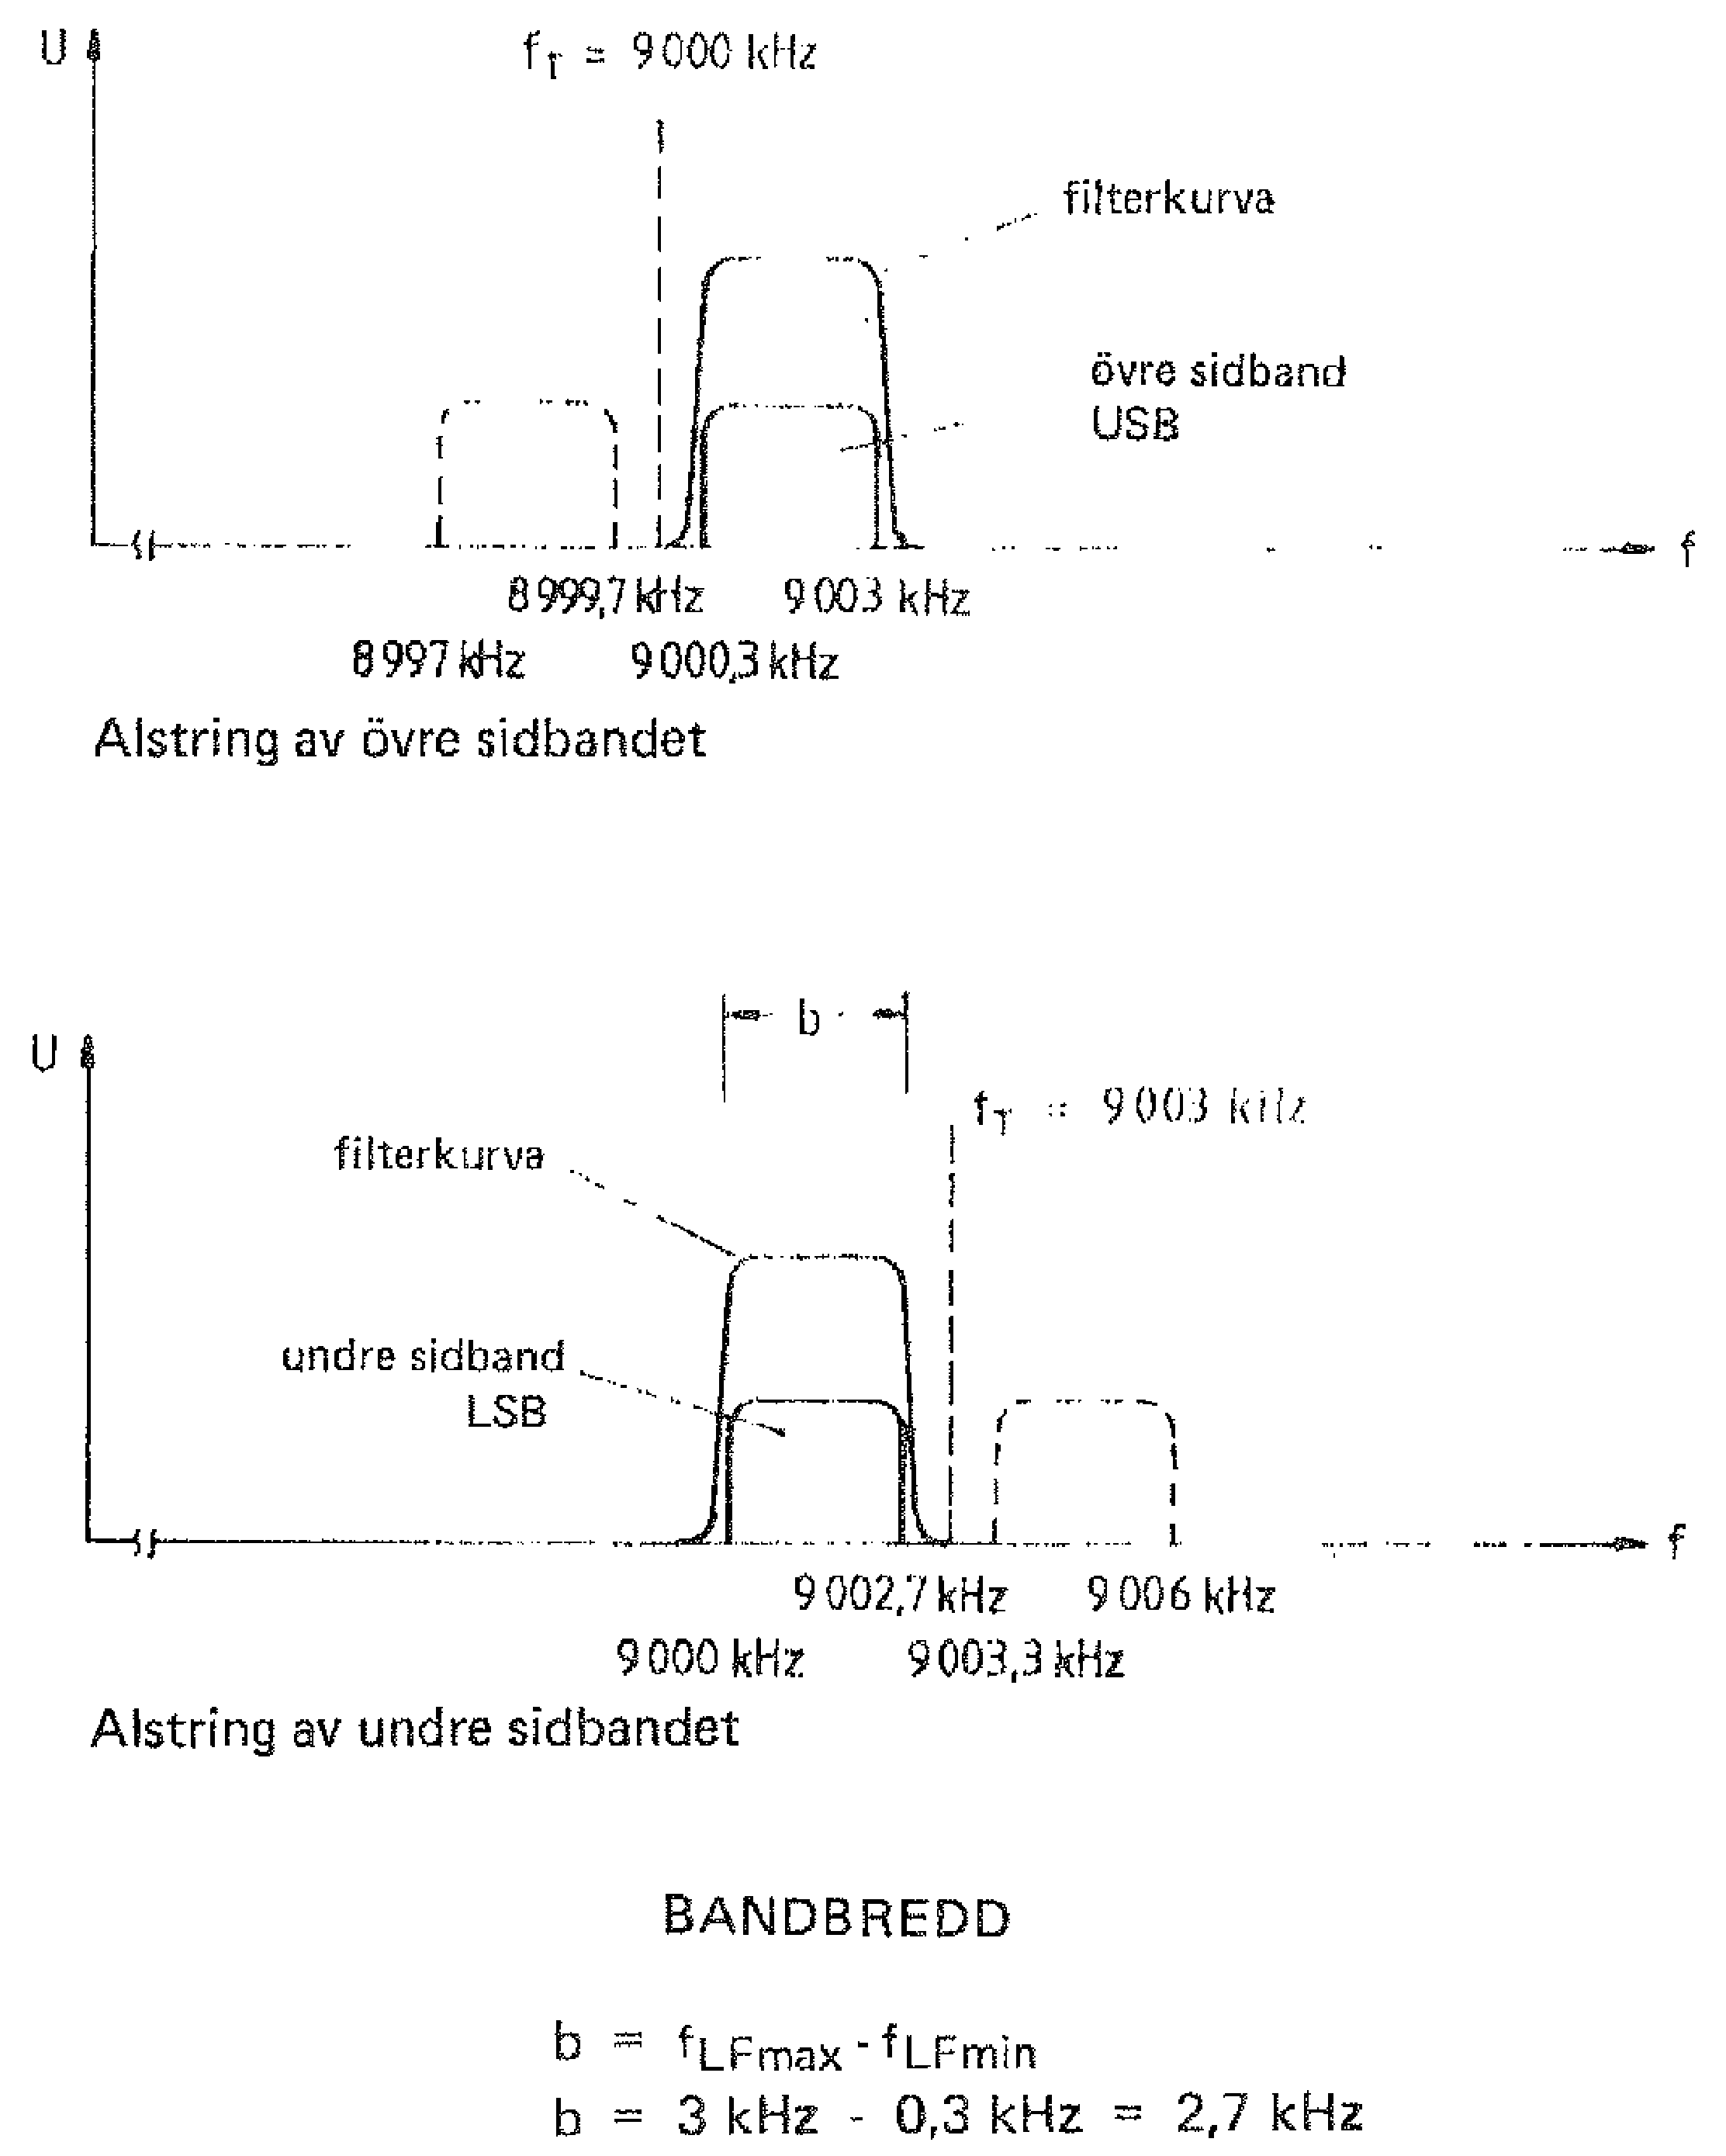
\includegraphics[width=\textwidth]{images/cropped_pdfs/bild_2_1-28.pdf}
\caption{Sidbandsval vid SSB}
\label{fig:BildII1-28}
\end{figure}

Bild \ref{fig:BildII1-28}.

Ett SSB-filter har ett passband av 9000,3--9003~kHz. Vid bärvågsfrekvensen 9000~kHz
sträcker sig det övre sidbandet från 9000,3--9003~kHz och släpps igenom. Däremot
blir bärvågsfrekvensen undertryckt.

Det undre sidbandet 8997--8999,7~kHz faller utanför filtrets passband och blir
också undertryckt.

Ska däremot det undre sidbandet kunna passera igenom samma filter, så måste
bärvågsfrekvensen höjas med 3~kHz, alltså till 9003~kHz. Då faller det undre
sidbandet, 9002,7--9000,0~kHz inom filtrets passband.

Det övre sidbandet 9003,3--9006,0~kHz faller nu utanför passbandet och blir
undertryckt.

\begin{figure}
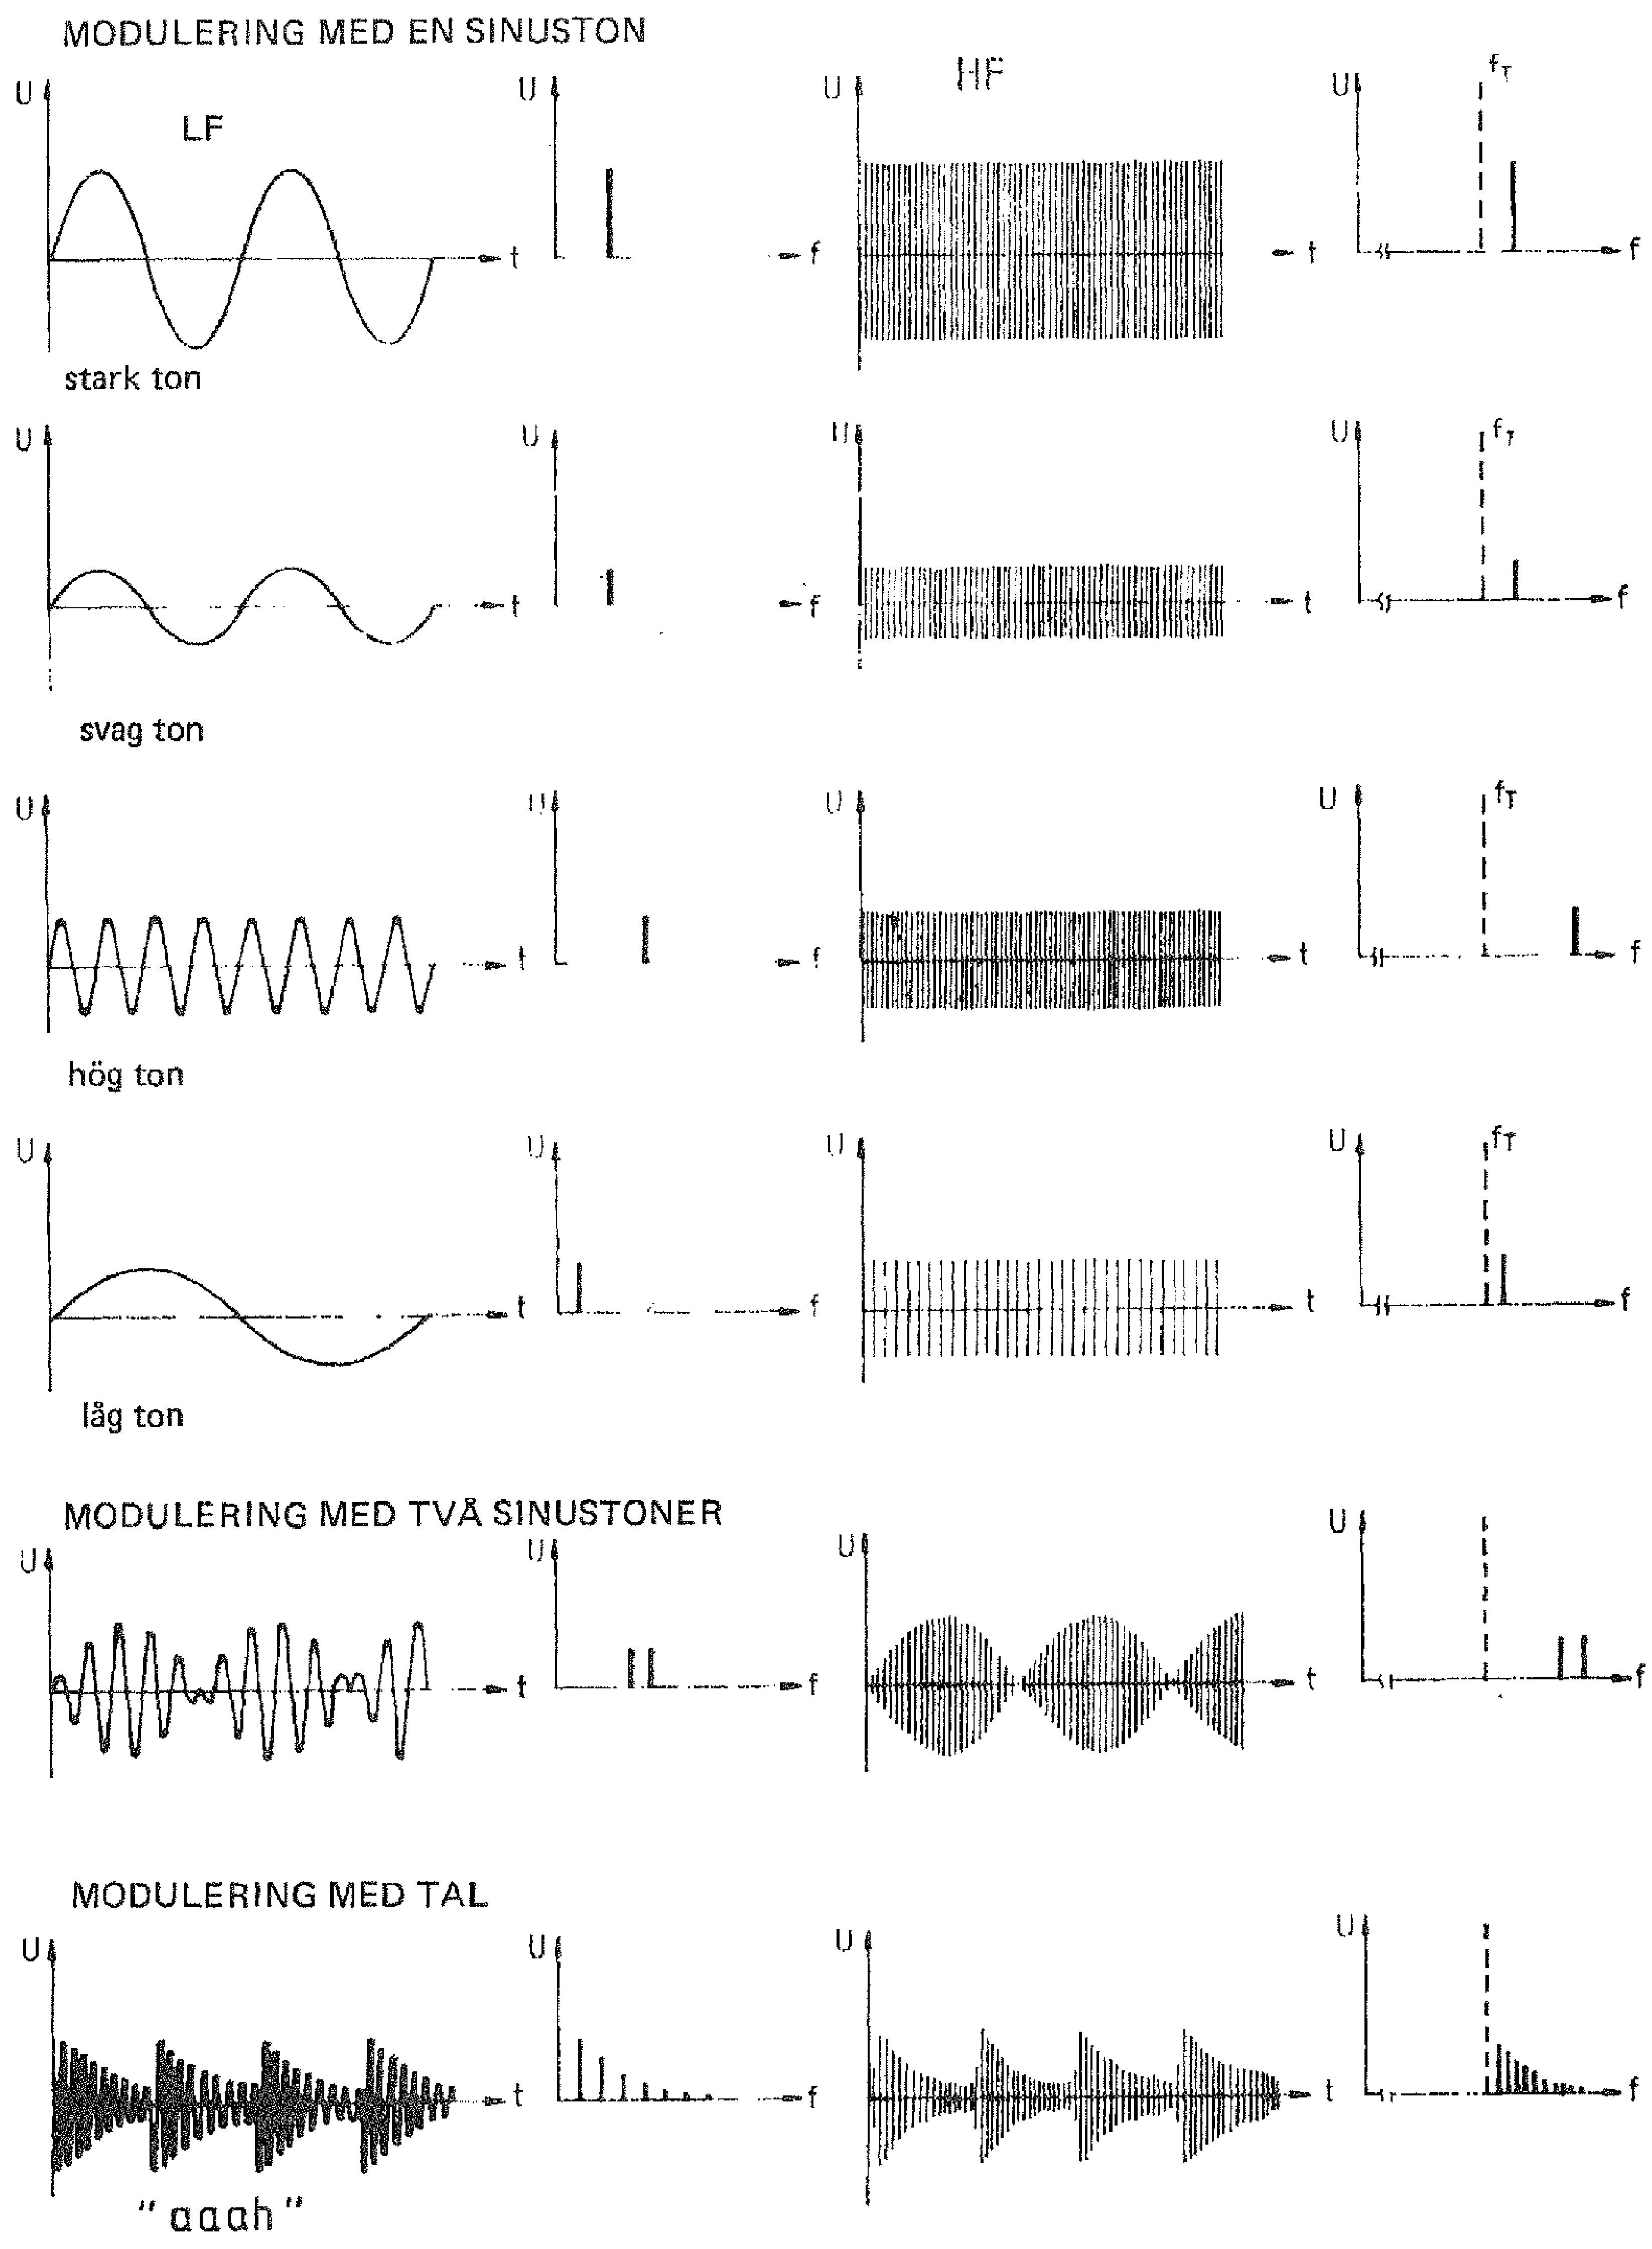
\includegraphics[width=\textwidth]{images/cropped_pdfs/bild_2_1-29.pdf}
\caption{Sidbandslägen vid SSB}
\label{fig:BildII1-29}
\end{figure}

Bild \ref{fig:BildII1-29}.

LF-signalens amplitud bestämmer amplituden på sidofrekvensen.

LF-signalens frekvens bestämmer sidofrekvensens avstånd från bärvågsfrekvensen
(bärvågen undertryckt).

Bandbredden på den utsända signalen är skillnaden mellan högsta och lägsta
modulerande frekvens i signalen:

t.ex. \(b = 3~kHz - 0,3~kHz = 2,7~kHz\)

\subsubsection{Fördelar med J3E-modulation}
Bra verkningsgrad vid J3E-modulation jämfört med vid A3E-modulation
(traditionell AM). Effekten i det utsända sidbandet motsvarar den i ett av
sidbanden vid A3E. Hela den utsända effekten finns alltså i ett enda sidband,
som överför hela informationen.

I sändningspauserna sänds ingen effekt ut. Bandbredden är mindre än hälften av
den vid A3E. Vid mottagning av en J3E-sändning (SSB) är det mindre besvär med
interferenstoner från J3E-sändningar på närliggande frekvenser, eftersom ingen
bärvåg och endast ett sidband sänds ut.

\subsubsection{Nackdelar med J3E-modulation}
J3E-modulation medför mera komplicerade apparater, både för mottagning och
sändning. En J3E-signal blir förvrängd och hörs i fel tonläge, om mottagaren
inte är inställd på exakt rätt frekvens.

\subsection{Vinkelmodulation}
\textbf{HAREC a.\ref{HAREC.a.1.8.3a}\label{myHAREC.a.1.8.3a}}
\index{vinkelmodulation}

Termen vinkelmodulation är samlingsnamnet för frekvensmodulation (FM) och
fasmodulation (PM). Ofta sägs utrustningar vara för frekvensmodulation, när de
antingen är för frekvens- eller fasmodulation. Det finns alltså skillnader och
likheter mellan dessa system, vilka emellertid inte är oberoende av varandra,
eftersom frekvensen i en signal inte kan varieras utan att fasen också
varieras, och vice versa.

Hur effektiv kommunikationen då är, beror mest på mottagningsmetoderna. I båda
fallen uppfattas ändringar i den mottagna signalens frekvens och fasläge.
Amplitudändringar uppfattas däremot inte. De flesta störningar -- särskilt
pulserande sådana som från tändningssystem -- kommer att därför att skiljas bort.

För att effektivt utnyttja fördelarna med vinkelmodulation, antingen det är
frekvens eller fasmodulation, behövs tillräckligt frekvensutrymme. Det innebär
att främst högre frekvensband kommer i fråga.

\subsection{Frekvensmodulation (även kallat FM)}
\textbf{HAREC
  a.\ref{HAREC.a.1.8.3b}\label{myHAREC.a.1.8.3b},
  a.\ref{HAREC.a.1.8.6d}\label{myHAREC.a.1.8.6d}
}
\index{frekvensmodulation}
\index{FM}

\begin{figure}
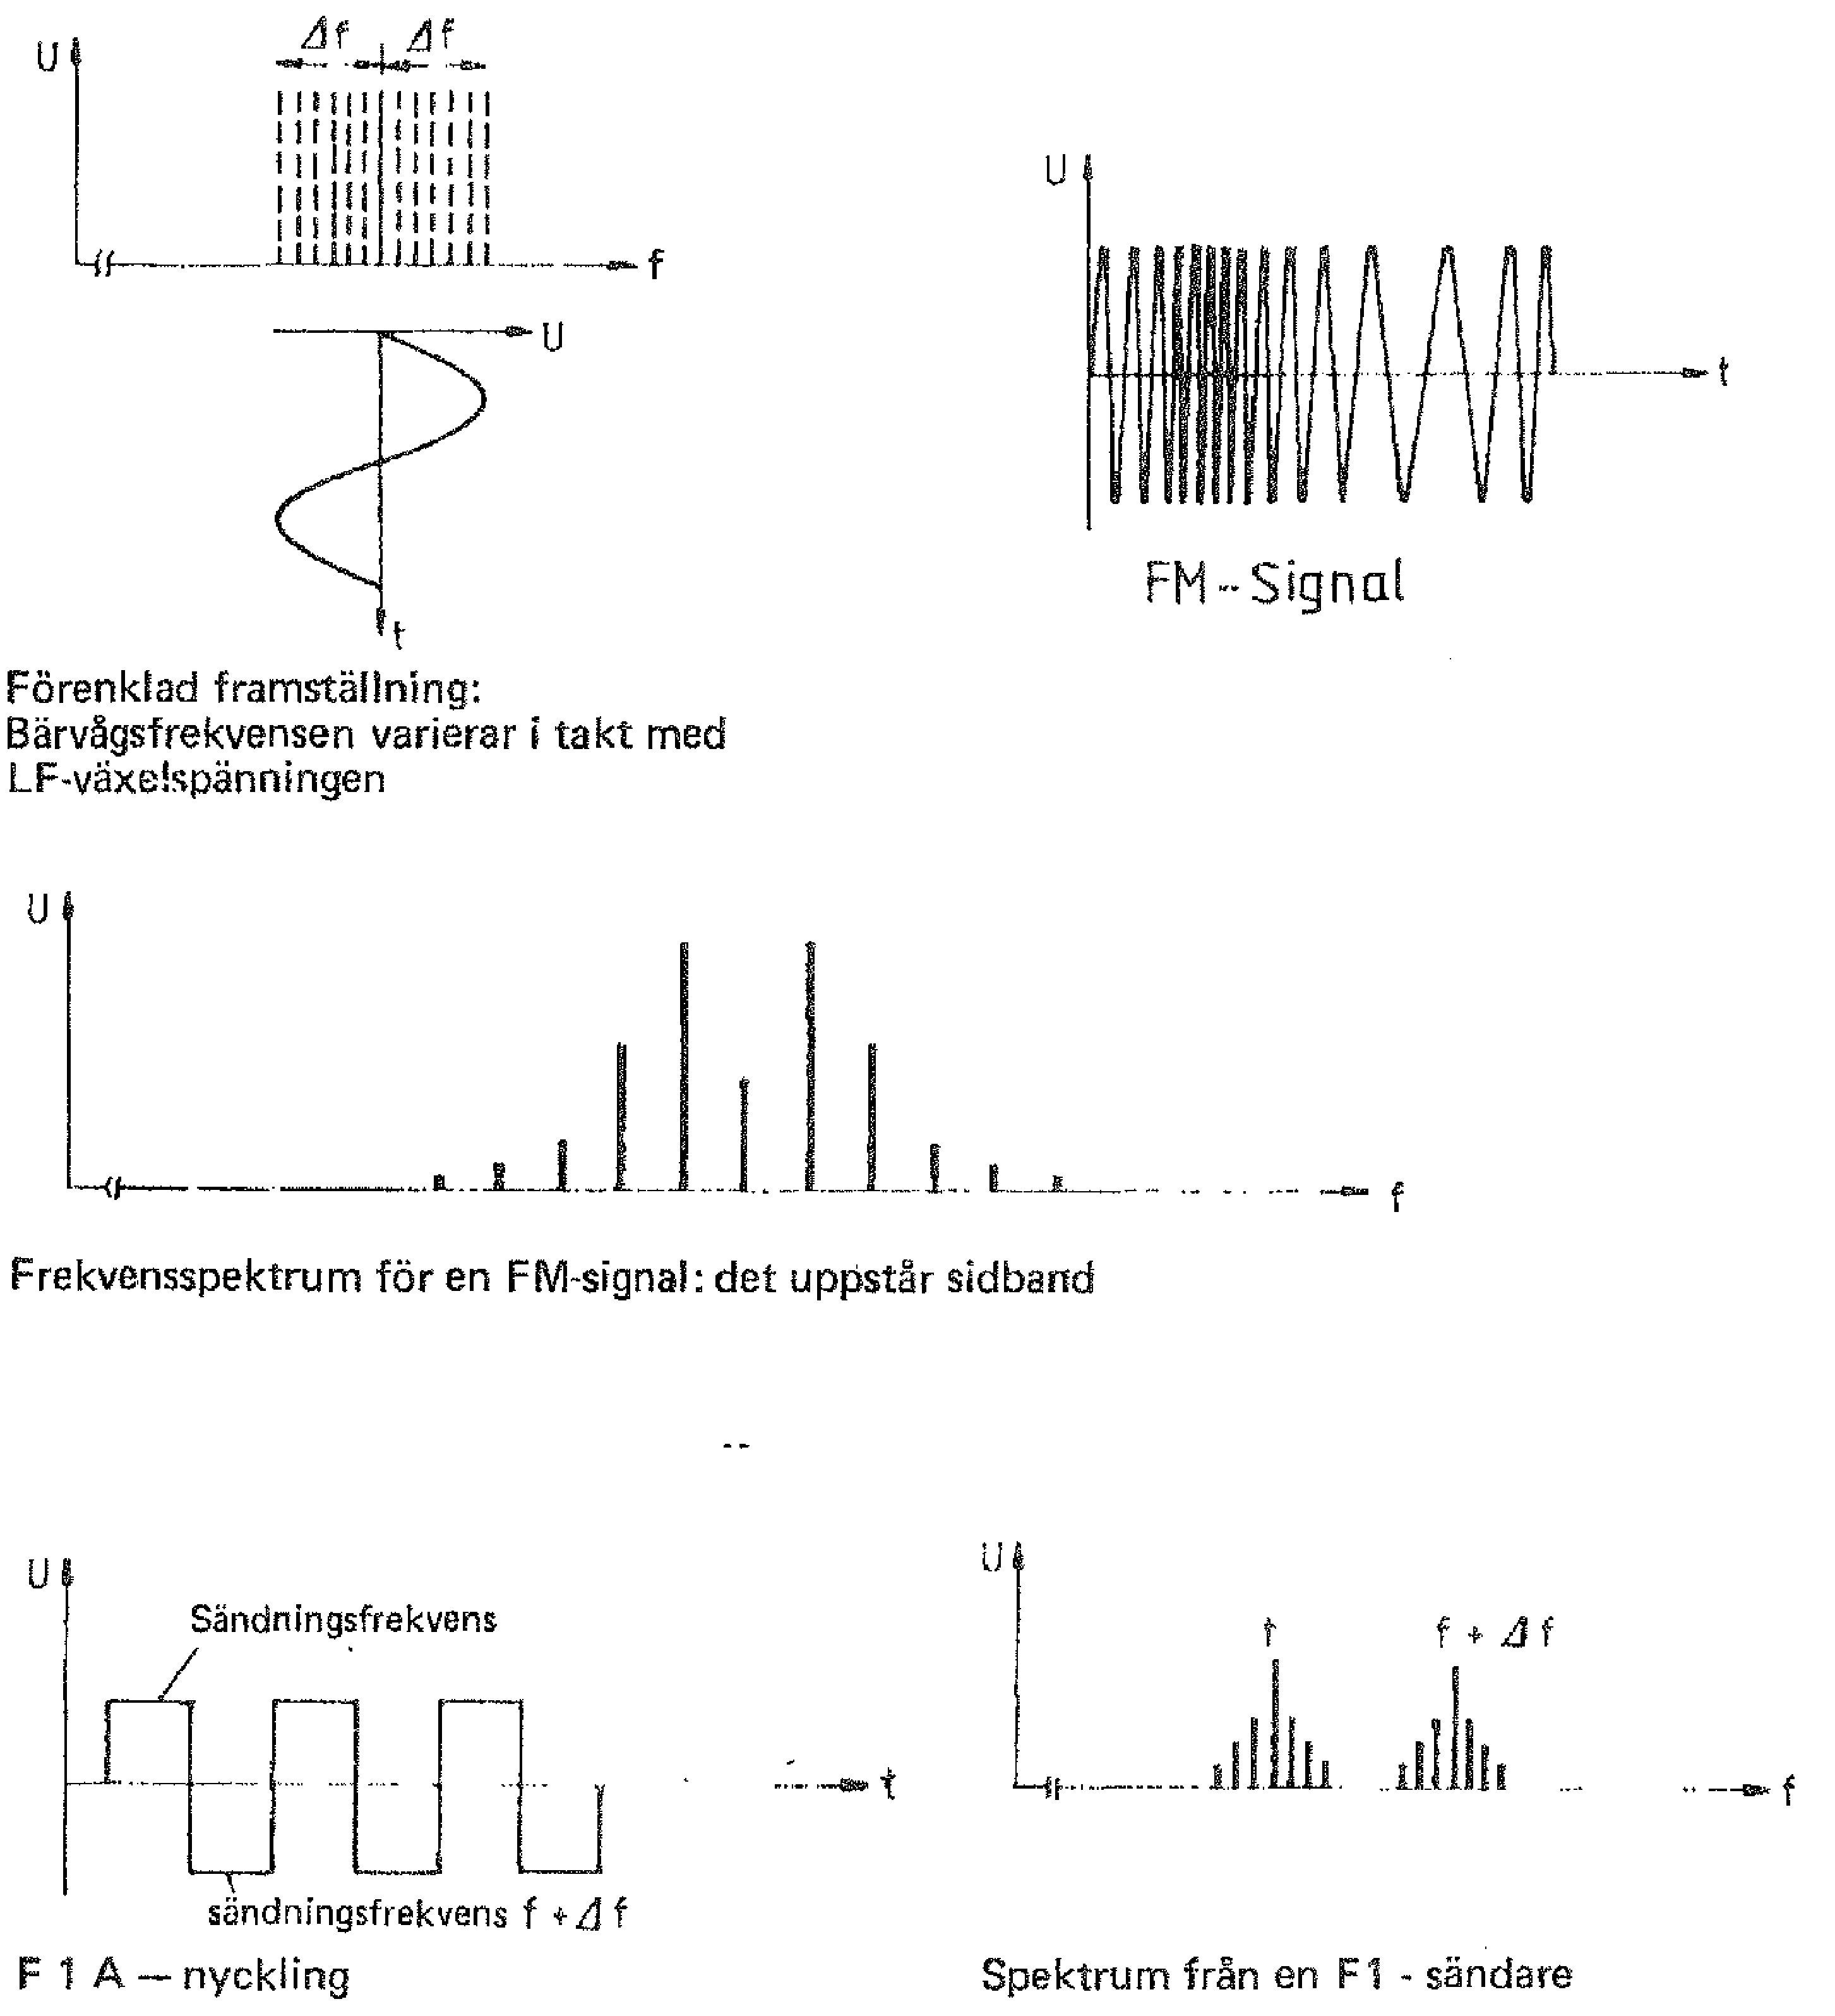
\includegraphics[width=\textwidth]{images/cropped_pdfs/bild_2_1-30.pdf}
\caption{Frekvensmodulation}
\label{fig:BildII1-30}
\end{figure}

Bild \ref{fig:BildII1-30} (överst och i mitten).

Vid frekvensmodulation varierar bärvågens frekvens i takt med den modulerande
signalens amplitud och polaritet. På bilden ökar bärvågens frekvens när den
modulerande signalen är positiv (första halvperioden) och minskar när den
modulerande signalen är negativ (andra halvperioden). Bilden visar att
perioderna i den modulerade bärvågen tar kortare tid (har högre frekvens), när
den modulerande signalen är positiv, och mertid (har lägre frekvens) när den
modulerande signalen är negativ. Bärvågen kommer alltså att pendla omkring ett
medelvärde, d.v.s. vara frekvensmodulerad.

Frekvensavvikelsen \(\Delta f\) (deviationen) från bärvågens vilofrekvens är
vid varje tillfälle proportionell till den modulerande signalens amplitud.
Sålunda är deviationen liten när den modulerande signalens amplitud är liten
och störst när amplituden når sitt toppvärde, antingen amplituden är positiv
eller negativ. Vid en modulationsfrekvens av 300~Hz varierar bärvågsfrekvensen
300 gånger per sekund, vid 3~kHz -- 3000 gånger per sekund.

Likspänningsnivåer kan överföras med FM, eftersom en motsvarande
frekvensavvikelse kan framställas.

Bilden visar också vad som oftast sägs, att bärvågsamplituden inte ändras av
modulationen. Detta är emellertid bara delvis sant, eftersom såväl
bärvågsamplitud som sidbandsamplitud varierar med modulationsindex, vilket
förklaras nedan.

\subsubsection{Sidbanden vid vinkelmodulation}

Vid AM produceras endast ett sidbandspar med samma innehåll, ett över och ett
under bärvågsfrekvensen. Vid vinkelmodulation, både vid FM och PM, produceras
däremot flera sidbandspar över och under bärvågsfrekvensen. Dessa sidband
uppträder på multiplerna av varje modulerande frekvens. Vid basband med samma
frekvensomfång har därför en vinkelmodulerad signal större bandbredd än en
AM-signal.

Vid vinkelmodulation beror antalet sidband på sambandet mellan den modulerande
frekvensen, frekvensdeviationen och modulationsindex.

\subsubsection{Bandbredden vid vinkelmodulation}

Bild \ref{fig:BildII1-30} (nederst).

Vi gör tankeexperimentet att en FM-sändare moduleras med en fyrkantsvåg.
Frekvensen kommer då att hoppa växelvis mellan frekvenserna \(f\) och
\(f + \Delta f\). Sättet kallas FSK (frekvensskiftnyckling) och används t.ex.
vid sändning av radiofjärrskrift (RTTY, AMTOR, Paketradio etc.).

Vi föreställer oss två sändare, som sänder varannan gång, varav den ena sänder
frekvensen \(f\) och den andra sänder \(f + \Delta f\). Båda sändarnas
HF-signaler kommer då att bilda ett frekvensspektrum, som förutom \(f\) och
\(f + \Delta f\) även innehåller sidofrekvenser.

Bredden på detta spektrum beror bl.a. på nycklingsfrekvensen. Eftersom en
fyrkantsvåg innehåller summan av dess grundfrekvens och övertoner, kommer alla
dessa toner att modulera vardera sändaren. De högsta modulerande
LF-frekvenserna alstrar sidofrekvenserna längst ut från vilofrekvensen.
LF-signalens frekvensspektrum påverkar alltså HF-signalens bandbredd.

Spektrum nederst i bilden är en förenklad framställning av
frekvensskiftnyckling.

Vid modulation med en sinussignal istället för med en fyrkantssignal, uppstår ett
frekvensspektrum som på överst i bilden.

\paragraph{Frekvensdeviation och modulationsindex}
\textbf{HAREC a.\ref{HAREC.a.1.8.4}\label{myHAREC.a.1.8.4}}
\index{frekvensdeviation}
\index{modulationsindex (m)}
\index{symbol!\(m\) modulationsindex}

\begin{figure}
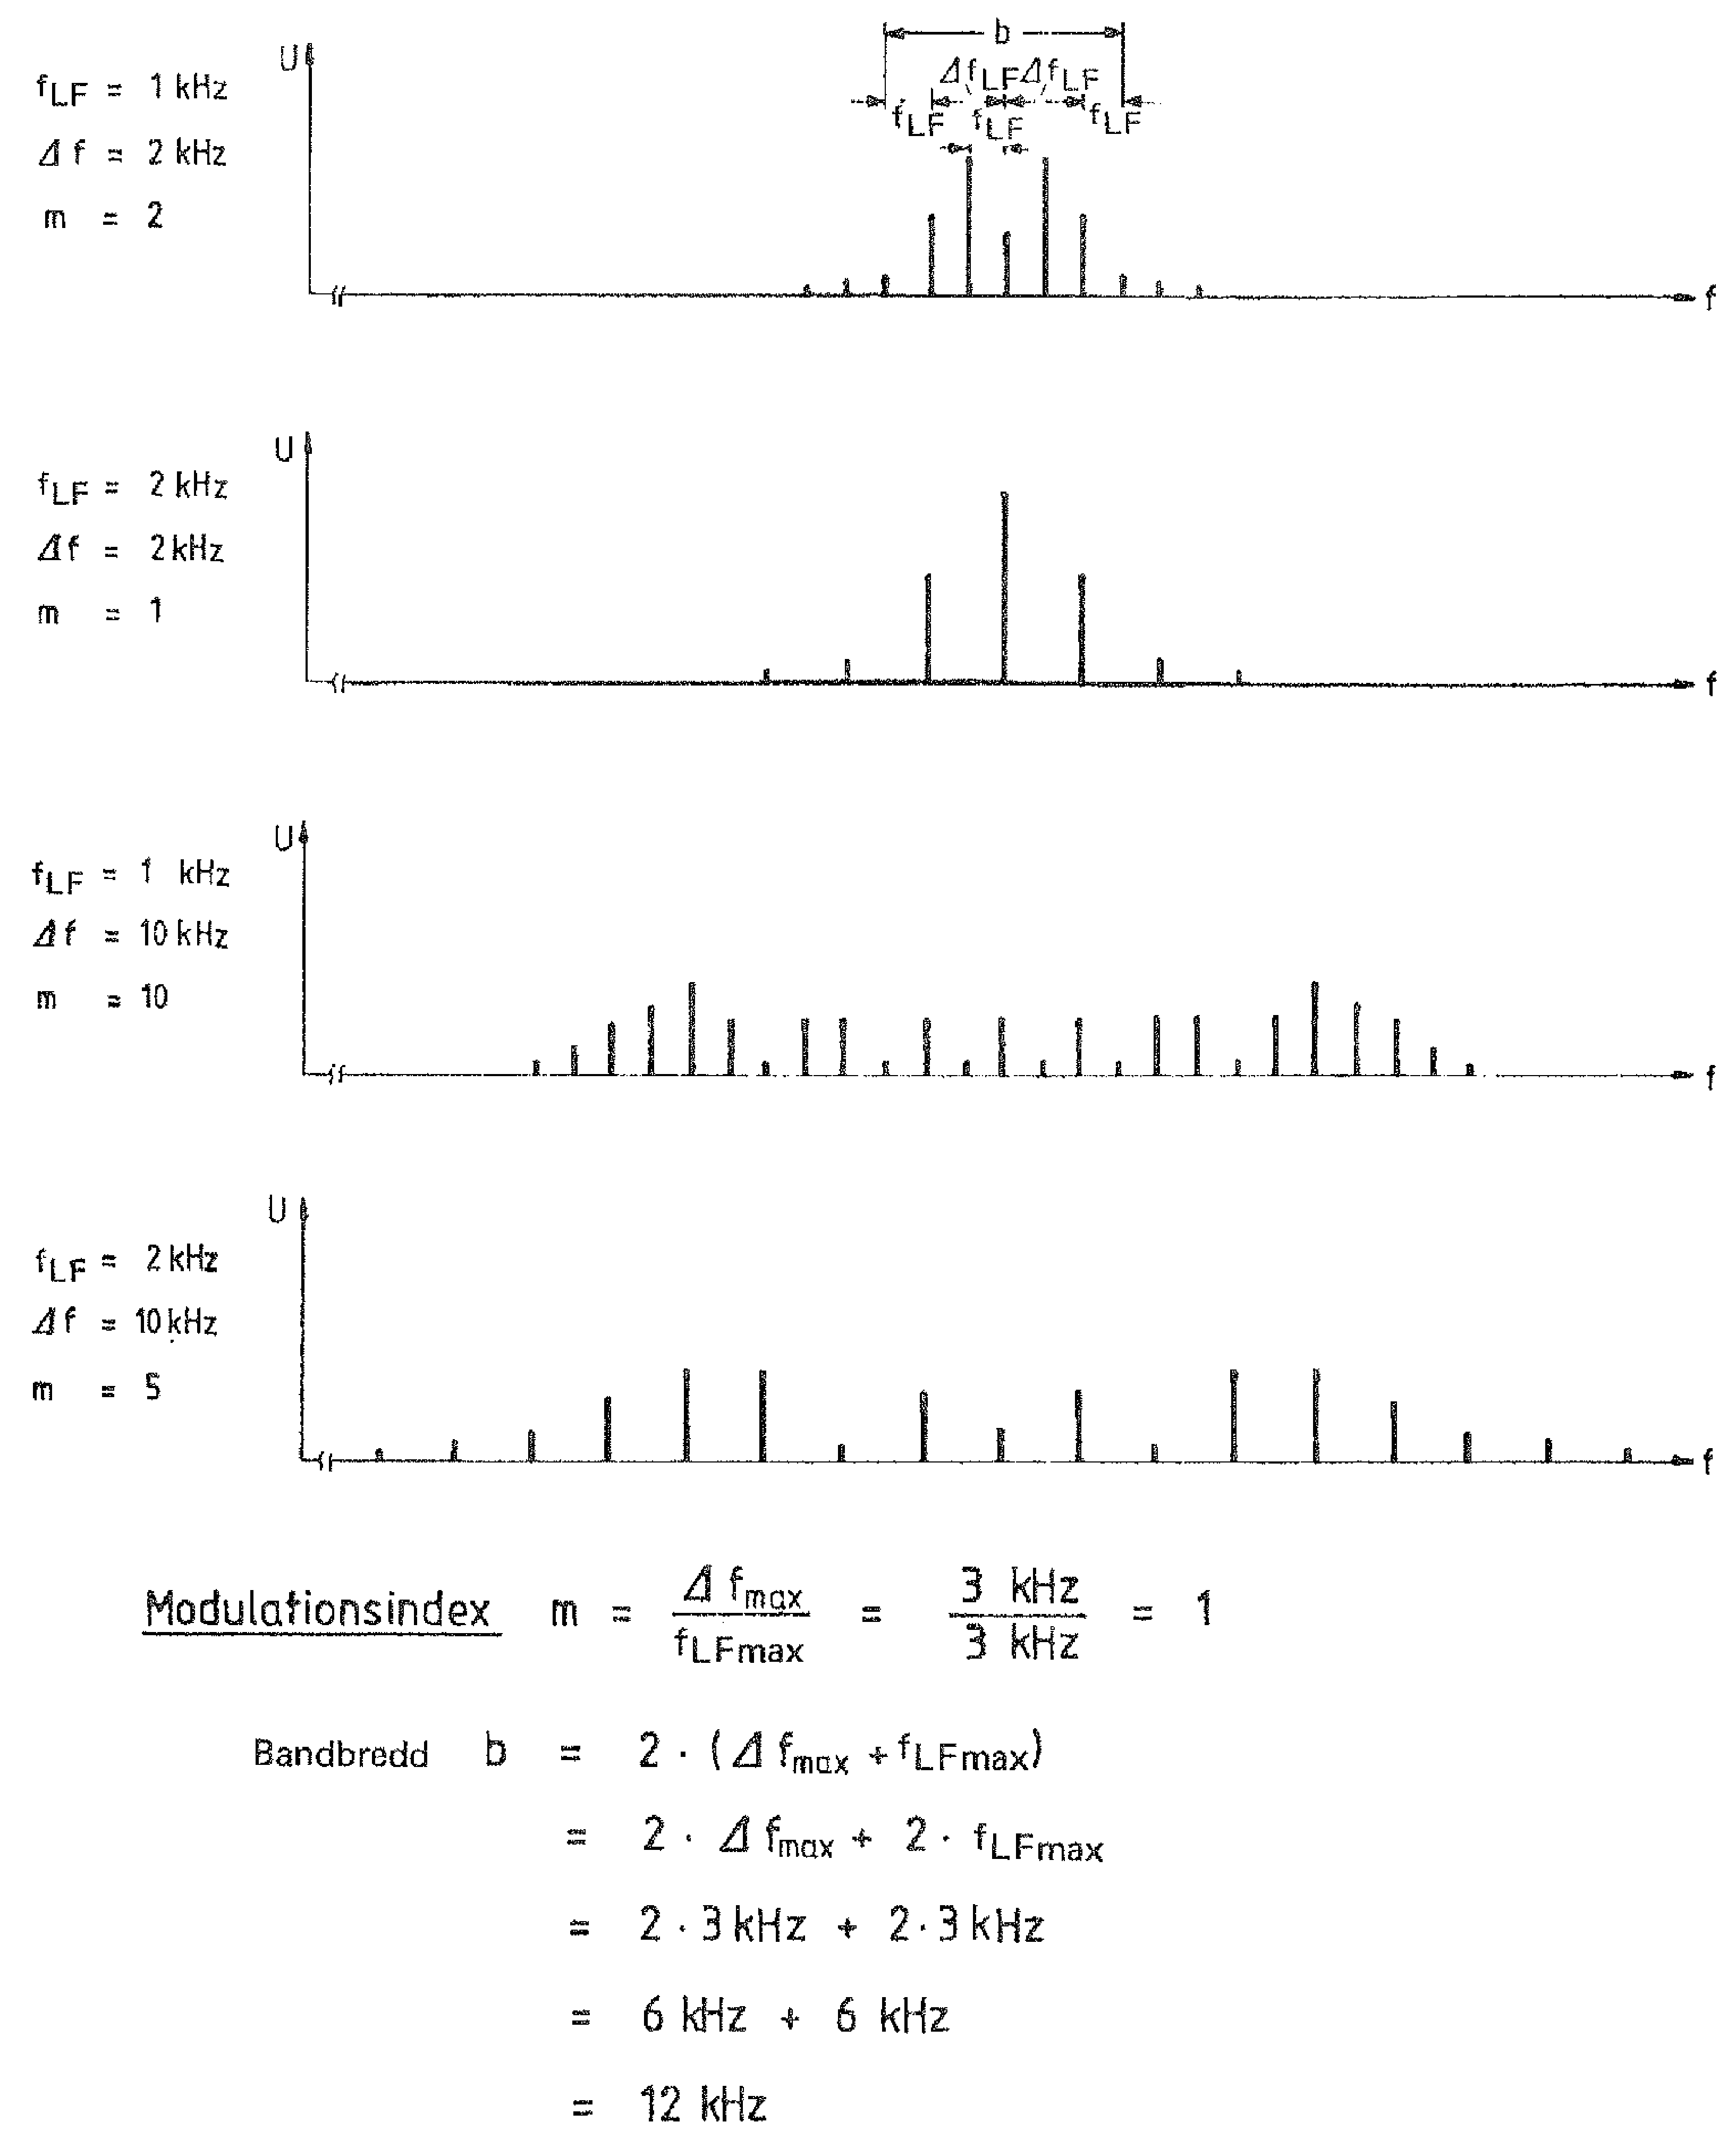
\includegraphics[width=\textwidth]{images/cropped_pdfs/bild_2_1-31.pdf}
\caption{Sidbandsspektrum vid FM-modulering med 1 sinuston}
\label{fig:BildII1-31}
\end{figure}

Bild \ref{fig:BildII1-31}.

Vid vinkelmodulation uppstår talrika sidofrekvenser, som beror av den
modulerande frekvensen \(f_{LF}\). Amplitudfördelningen mellan sidofrekvenserna
står i förhållande till deviationen, varvid deras amplitud blir mindre desto
längre bort från bärvågen de är.

I praktiken anses en sidofrekvens försumbar när dess amplitud är mindre än 1~\%
av amplituden för omodulerad bärvåg.

För beräkning av bandbredden används begreppet modulationsindex m, vilket är
kvoten av maximal deviation \(\Delta f\) och högsta frekvensen \(f_{LF}\).

\(m = \dfrac{\Delta f_{max}}{f_{LFmax}}\)

Inom amatörradion är det vanligt att arbeta med \(\Delta f_{max} = 3 kHz\) och
\(f_{LFmax} = 3 kHz\), d.v.s. \(m = 1\).

Vid modulationsindex \(m = 1\), gäller följande
formel för bandbredden \(b\)

\(b = 2 \cdot ( \Delta f_{max} + f_{LFmax}) = 2 \cdot \Delta f_{max}
 + 2 \cdot f_{LFmax}\)

Med ovan nämnda värden blir bandbredden \(b = 2 \cdot (3 kHz + 3 kHz)
 = 12 kHz\)

Bandbredden ökar således både med ökande deviation och ökande modulerande
frekvens. För att inte interferera med trafik på grannkanalerna måste såväl
deviation som frekvensen på den modulerande signalen begränsas. En
deviationsbegränsare begränsar amplituden på denna signal. Ett lågpassfilter
reducerar den distorsion, som uppstår av begränsningen. Vidare undertrycks
modulerande frekvenser högre än 3~kHz, vilket är tillräckligt för överföring
av tal.

\paragraph{Jämförelse}

En VHF-rundradiosändare är tilldelad ett större frekvensutrymme och kan därför
använda mycket större bandbredd

Där är \(\Delta f_{max} = 75 kHz\) och \(f_{LFmax} =15 kHz\), därmed är
\(m = \frac{75}{15} = 5\) och \(b = 2 \cdot (75 + 15) = 180 kHz\).

Som framgår av tabellen på nästa uppslag varierar bärvågens liksom
sidofrekvensernas inbördes amplitud med modulationsindex. Detta ska jämföras
med AM där bärvågens amplitud är konstant och endast sidbandens amplitud
varierar.

Vid vinkelmodulation utsläcks bärvågen \(A_0\) vid modulationsindex 2.404. Den
blir sedan ''negativ'' vid högre index, vilket betyder att den återkommer, men
att dess fasläge blir omvänt. I vinkelmodulation tas energin i sidbanden från
bärvågen, vilket innebär att den totala effekten förblir densamma oavsett
modulationsindex.

\paragraph{Kännetecken för sändningsslaget F3E (FM)}
\index{F3E}

Fördelar: F3E-sändaren är enkel till sin uppbyggnad och hög överföringskvalitet
uppnås vid stor bandbredd, störningar från amplitudmodulerade signaler t.ex.
tändgnistor undertrycks i mottagaren.

Nackdelar: En relativt stor bandbredd behövs för överföring av ett basband med
stort frekvensomfång. Sändaren måste avge full effekt, även när modulation inte
sker.

\begin{table*}[h]
\begin{center}
\begin{tabular}{ll|l|l|l|l|l|l|l|l|}
\cline{3-9}
&\multicolumn{1}{l}{}  & \multicolumn{7}{|c|}{Modulationsindex} \\ \cline{3-9}
&\multicolumn{1}{l|}{}  &   1   &   2   &    3   &    4   &    5   &    6   &    7   \\ \hline
\multicolumn{1}{|c|}{\multirow{11}{*}{\rotatebox[origin=c]{90}{Relativ amplitud på}}}&\(A_0\) & 0.765 & 0.224 & -0.260 & -0.397 & -0.178 &  0.151 &  0.300 \\
\multicolumn{1}{|c|}{}&\(A_1\) & 0.440 & 0.577 &  0.334 & -0.066 & -0.328 & -0.277 & -0.005 \\
\multicolumn{1}{|c|}{}&\(A_2\) & 0.115 & 0.353 &  0.486 &  0.364 &  0.047 & -0.243 & -0.301 \\
\multicolumn{1}{|c|}{}&\(A_3\) & 0.020 & 0.129 &  0.309 &  0.430 &  0.365 &  0.115 & -0.168 \\
\multicolumn{1}{|c|}{}&\(A_4\) &       & 0.034 &  0.132 &  0.281 &  0.391 &  0.358 &  0.158 \\
\multicolumn{1}{|c|}{}&\(A_5\) &       & 0.016 &  0.043 &  0.132 &  0.261 &  0.362 &  0.348 \\
\multicolumn{1}{|c|}{}&\(A_6\) & \multicolumn{2}{c|}{} &  0.011 &  0.049 &  0.131 &  0.246 &  0.339 \\
\multicolumn{1}{|c|}{}&\(A_7\) & \multicolumn{3}{c|}{} &  0.015 &  0.053 &  0.130 &  0.234 \\
\multicolumn{1}{|c|}{}&\(A_8\) & \multicolumn{4}{c|}{}           &  0.018 &  0.057 &  0.128 \\
\multicolumn{1}{|c|}{}&\(A_9\) & \multicolumn{4}{c}{} &        &  0.021 &  0.059 \\
\multicolumn{1}{|c|}{}&\(A_{10}\) & \multicolumn{5}{c}{Tomma fält för \(A_n\) under 0.01 (1 \%)} &  &  0.024 \\ \hline
\end{tabular}
\end{center}
\caption{Relativa amplituden på bärvåg $A_0$ och sidofrekvenser $A_1$--$A_{10}$ vid
modulationsindex 1--7 (Vid omodulerad bärvåg är modulationsindex 0. Då är
bärvågens relativa amplitud 1,0)}
\end{table*}


\subsection{Fasmodulation (även kallat PM)}
\index{fasmodulation}
\index{PM}

Vid fasmodulation varierar bärvågens fasläge i förhållande till ett
referensvärde. Vid PM är frekvensändringen -- deviationen -- direkt proportionell
till hur snabbt fasläget på den modulerande frekvensen ändras och till den
totala fasändringen. Hastigheten på fasändringen är direkt proportionell till
frekvensen på den modulerande frekvensen och till den momentana amplituden på
den modulerande signalen.

Det betyder att deviationen i PM-system ökar både med den momentana amplituden
och frekvensen på den modulerande signalen. Detta att jämföras med FM-system där
deviationen är proportionell till den momentana amplituden på den modulerande
signalen.

I PM-system uppfattar demodulatorn i mottagaren endast momentana ändringar i
bärvågsfrekvensen. Till skillnad från vid FM, så kan därför ändringar i
likspänningsnivåer överföras endast om en fasreferens används.

Med konstant amplitud på insignalen till modulatorn, så är vid PM
modulationsindex konstant oavsett modulerande frekvens, medan vid FM
modulationsindex varierar med den modulerande frekvensen.

\subsection{Frekvens- och fasmodulation jämförs}

\begin{itemize}
\item Frekvensmodulation (FM) alstras genom att sändarens oscillatorfrekvens
varieras (devieras) i takt med den modulerande signalen (t.ex. tal). Det gör man
genom att variera resonansfrekvensen i den svängningskrets som styr
oscillatorfrekvensen.

\item Fasmodulation (PM) alstras vanligen genom att efter sändaroscillatorn
variera den modulerande signalens fasläge i förhållande till en omodulerad
bärvåg -- s.k. fasmodulering. Det gör man genom att variera resonansfrekvensen i
en svängningskrets efter oscillatorn- d.v.s. utan att påverka
oscillatorfrekvensen.

\item I båda fallen ändrar man alltså resonansfrekvensen i en svängningskrets i
takt med frekvensen i den modulerande spänningen, men att denna krets har olika
placering i FM-sändare respektive PM-sändare.

\item I sändaren alstras det i båda fallen utfrekvenser som devierar från
oscillatorns vilofrekvens. Graden av deviation skiljer emellertid vid FM och PM.
Vid FM är deviationen proportionell mot amplituden på den modulerande
underbärvågen medan deviationen vid PM är proportionell mot produkten av den
modulerande underbärvågens amplitud och frekvens.

\item Den hörbara skillnaden mellan FM och PM är därför en annorlunda
frekvensgång. Vid samtidig användning av PM-sändare och FM-mottagare är det
alltså lämpligt att justera frekvensgången i PM-sändarens modulator, lämpligen
med 6~dB dämpning per oktav ökad frekvens.
\end{itemize}

\subsection{Pulsmodulation}
\index{pulsmodulation}
\index{PWM}
\index{PAM}
\index{PPM}

Pulsmodulation används mest i mikrovågsområdet. Pulsmodulerade signaler sänds
vanligen som en serie korta pulser åtskilda av relativt långa pauser utan
modulering.

En typisk sändning kan bestå av pulser med en längd av 1 \(\mu\)s och en
frekvens av 1000~Hz. Toppeffekten på en pulssändning är därför mycket högre än
dess medeleffekt

Före WARC 79 var symbolen för all pulssändning P. Därefter används P endast för
omodulerade pulståg. Annan pulsmodulation har följande symboler

\begin{description}
\item[K] -- puls-/amplitudmodulation (PAM)
\item[L] -- pulsviddmodulation (PWM)
\item[M] -- pulsposition/fasmodulation (PPM)
\item[Q] -- vinkelmodulation under pulsen
\item[V] -- kombination av dessa eller annat sätt.
\end{description}

\begin{table*}[h]
\begin{center}
\begin{tabular}{|l|l|l|l|l|}
\hline
Sändningsslag & Amplituden på & Tonhöjden på & Bandbredden b      & För stor amplitud \\
              & LF-signalen   & LF-signalen  & förhåller sig till & på LF-signalen \\
              & påverkar      & påverkar     &                    & medför \\ \hline
A3E (AM) & amplituden i   & sidofrekvenser- & LF-signalens    & övermodulering \\
         & båda sidbanden & nas avstånd    & högsta frekvens & och för stor bandbredd \\
         &                & från bärvågen  & & \\
J3E (SSB)& amplituden på  & sidofrekvenser- & skillnaden mellan & för stor bandbredd,\\
         & utsänt sidband & nas avstånd    & LF-signalens      & överstyrning av\\
         &                & från bärvågen  & högsta och lägsta & förstärkarsteg\\
         &                &                & frekvens          & \\
F3E (FM) & deviationen    & hastigheten på & dubbla summan     & för stor deviation,\\
         &                & bärvågens      & av största devia- & för stor bandbredd\\
         &                & frekvens-      & tion och högsta   & \\
         &                & ändring        & LF-frekvens       & \\ \hline
\end{tabular}
\end{center}
\caption{Jämförelse mellan några vanliga sändningsslag inom amatörradio}
\end{table*}

\subsection{Digital modulationer}
\textbf{HAREC a.\ref{HAREC.a.1.8.8}\label{myHAREC.a.1.8.8}}
\index{digital modulation}

Utöver de klassiska analoga modulationsmetoder finns ett antal digitala
modulationsformer. De är anpassade för transmission av binärt data. I viss mån
kan CW ses som digital modulation där en 0 moduleras utan bärvåg och 1 moduleras
med bärvåg. Det finns dock flera andra modulationsmetoder som FSK, 2-PSK/BPSK,
4-PSK och QAM som presenteras i följande delavsnitt.

\subsubsection{Frekvensskift modulation -- FSK}
\textbf{HAREC a.\ref{HAREC.a.1.8.8a}\label{myHAREC.a.1.8.8a}}
\index{frekvensskift modulation}
\index{Frequency Shift Keying (FSK)}
\index{FSK}
\index{frekvensmodulation}
\index{FM}
\index{GFSK}
\index{Gaussiskt filter}
\index{C4FM}
\index{JT65}
\index{JT9}

\emph{Frekvensskift modulation} (eng. \emph{Frequency Shift Keying (FSK)})
skiljer sig från CW modulationen med att den ändrar frekvensen, dvs. är en
variant av frekvensmodulation. I den enklaste formen, binär FSK, så växlar man
mellan 2 frekvenser, där en frekvens får representera 0 och den andra får
representera 1. Denna metod har används för modem på telefon-förbindelser,
så som Bell 103.

Eftersom varje växling mellan frekvenser ger avbrott i bägge signalerna,
likt nycklingen i CW, så kommer de skapa sidband. Av det skälet filtrerar man
gärna signalen, och använder man ett Gaussiskt filter får man Gaussian Frequency
Shift Keying (GFSK) som används av t.ex. GSM telefoni.

Man kan använda fler än 2 frekvenser, t.ex. används 4 frekvenser i Continuous
4 level FM (C4FM) i Phase 1 radios i Project 25 samt Fusion.

Frekvensskift används även för att sända långsamma meddelanden där JT65
använder 65 frekvenser den skiftar mellan, medans JT9 använder 9 frekvenser.

\subsubsection{Binär fasskift modulation -- 2-PSK \& BPSK}
\textbf{HAREC a.\ref{HAREC.a.1.8.8b}\label{myHAREC.a.1.8.8b}}
\index{binär fasskift modulation}
\index{fasskift modulation!binär}
\index{2-PSK}
\index{fasskift modulation!2-PSK}
\index{BPSK}
\index{fasskift modulation!BPSK}
\index{Costas loop}

Istället för att modulera frekvensen kan man modulera polariteten eller fasen.
En sådan modulationsform är \emph{binär fasskift modulation} (eng
\emph{Binary Phase Shift Keying (BPSK)} eller \emph{2-state Phase Shift Keying
(2-PSK)}. Förenklat kan man säga att bärvågen moduleras med +1 eller -1,
ofta med +1 representerande 0 och -1 representerande 1.

En nackdel med BPSK är att blir polariteten förväxlad så kommer meddelandet
att bli inverterat, dvs. 0 blir 1 och 1 blir 0. BPSK behöver därför också
kompletteras med annan digital modulation för att hantera polariteten, något
som i allmänhet kan åstadkommas enkelt.

BPSK används t.ex. av satellitnavigationssystem som GPS, GLONASS och Galileo.
För att återvinna BPSK behöver man ofta en speciell variant av PLL-loop känd
som \emph{Costas loop}, eftersom en normal PLL-loop klarar inte av
teckenändringarna på signalen.

\subsubsection{Fyrnivå fasskiftmodulation -- 4-PSK}
\textbf{HAREC a.\ref{HAREC.a.1.8.8c}\label{myHAREC.a.1.8.8c}}
\index{4-PSK}
\index{fasskift modulation!4-PSK}
\index{kvadratur-modulering}
\index{quadrature modulation}
\index{in phase}
\index{quadrature}
\index{I/Q modulation}

Fasskiftmodulation kan även göras med flera nivåer, och 4 olika fas-lägen
kan användas och kallas då för \emph{fyrnivå fasskiftmodulation} (eng
\emph{4-state Phase Shift Keying (4-PSK)}.

Istället för 180 graders fas-skift (0 och 180 grader) som 2-PSK/BPSK använder
så använder man 360/4 dvs. 90 graders fas-skift mellan symbolerna.
Ett effektivt sätt att avkoda det är att göra \emph{kvadratur-modulering}
(eng. \emph{quadrature modulation}) där man modulerar en signal till två
komponenter, i fas (eng. \emph{In Phase (I)}) och kvadratur (eng.
\emph{Quadrature (Q)}), ofta kallat I/Q modulering.

De fyra fas-lägena kan nu enkelt förklaras som amplituder i de olika fas-lägena
som anges av tabell \ref{tab:4-PSK}.

\begin{table*}[h]
\begin{center}
\begin{tabular}{|r|r|r|r|}
\hline
Symbol & Vinkel & I & Q \\ \hline
0 &   0 & +1 &  0 \\
1 &  90 &  0 & +1 \\
2 & 180 & -1 &  0 \\
3 & 270 &  0 & -1 \\ \hline
\end{tabular}
\end{center}
\caption{4-PSK i kvadratur-modulering}
\label{tab:4-PSK}
\end{table*}

Amplituden är densamma för alla 4 symbolerna, men med olika vinkel.
I likhet med 2-PSK/BPSK behöver man återvinna fasen och sedan kunna avgöra
vad som är 0 grader, men givet att det görs i den övriga modulationen så
kan informationen avkodas korrekt.

\subsubsection{Kvadratur-amplitud modulation -- QAM}
\textbf{HAREC a.\ref{HAREC.a.1.8.8d}\label{myHAREC.a.1.8.8d}}
\label{QAM}
\index{kvadratur-amplitud modulation}
\index{QAM}
\index{QAM-16}
\index{DAB}
\index{DVB-T}
\index{DVB-T2}
\index{Wi-Fi}

Medans fasskiftnings kan göras för fler fas-steg har man funnit att det är
inte lika smidigt för högre upplösningar. Redan vid 8 steg behöver man ha
I och Q värden som är \(\sqrt{1/2}\), vilket iofs går att approximera.
En smidigare modulationsform är istället att låta även amplituden variera,
och genom att låta några bitar modulera I och några bitar modulera Q så kan
man enkelt få en konsistent modulations-mappning som är effektiv att
implementera. Denna kallar man \emph{kvadratur-amplitud modulation} (eng
\emph{Quadrature Amplitude Modulation (QAM)}).

Ofta benämner man olika varianter med antalet olika positioner, så att QAM-16
har 16 olika fas-amplitud-lägen. Ett exempel på hur QAM-16 kan moduleras finns
i tabell \ref{tab:QAM-16}.

\begin{table*}[h]
\begin{center}
\begin{tabular}{|r|r|r|r|r|r|r|}
\hline
Symbol & Isym & Qsym & Amplitud      & Vinkel &  I &   Q \\ \hline
     0 &    0 &    0 & \(3\sqrt{2}\) &    +45 & +3 &  +3 \\
     1 &    0 &    1 & \(\sqrt{10}\) &    +72 & +3 &  +1 \\
     2 &    0 &    2 & \(\sqrt{10}\) &   +108 & +3 &  -1 \\
     3 &    0 &    3 & \(3\sqrt{2}\) &   +135 & +3 &  -3 \\
     4 &    1 &    0 & \(\sqrt{10}\) &    +18 & +1 &  +3 \\
     5 &    1 &    1 &  \(\sqrt{2}\) &    +45 & +1 &  +1 \\
     6 &    1 &    2 &  \(\sqrt{2}\) &   +135 & +1 &  -1 \\
     7 &    1 &    3 & \(\sqrt{10}\) &   +162 & +1 &  -3 \\
     8 &    2 &    0 & \(\sqrt{10}\) &   +342 & -1 &  +3 \\
     9 &    2 &    1 &  \(\sqrt{2}\) &   +315 & -1 &  +1 \\
    10 &    2 &    2 &  \(\sqrt{2}\) &   +225 & -1 &  -1 \\
    11 &    2 &    3 & \(\sqrt{10}\) &   +198 & -1 &  -3 \\
    12 &    3 &    0 & \(3\sqrt{2}\) &   +225 & -3 &  +3 \\
    13 &    3 &    1 & \(\sqrt{10}\) &   +252 & -3 &  +1 \\
    14 &    3 &    2 & \(\sqrt{10}\) &   +288 & -3 &  -1 \\
    15 &    3 &    3 & \(3\sqrt{2}\) &   +315 & -3 &  -3 \\ \hline
\end{tabular}
\end{center}
\caption{Exempel på QAM-16 i kvadratur-modulering}
\label{tab:QAM-16}
\end{table*}

Medans både amplituder och vinklar kan kännas udda, så är det enkelt att
mappa bitarna över till I och Q amplituder via Isym och Qsym delarna av
symboler.

QAM-modulering används av DAB, DVB-T, DVB-T2, Wi-Fi, mikrovågslänkar och många
andra moderna system. Mikrovågslänkar använder upp till QAM-2048 idag.
En fördel med QAM-moduleringen är att det är enkelt att få samma avstånd
mellan de olika symbol-positionerna, och därmed kan också modulationen anpassas
till störningen. Detta nyttjas av många moderna modulations-system så att
QAM-modulationen anpassas utifrån mottagarens rapportering om störning.
Denna dynamiska anpassning gör att kommunikationen kan upprätthållas även om
kapaciteten tillåts variera.

\subsection{Digital modulation}
\textbf{HAREC a.\ref{HAREC.a.1.8.9}\label{myHAREC.a.1.8.9}}
\index{digital modulation}

Digital modulation innebär också att signalerna som sänds har lite andra
egenskaper än de analoga. Istället för varierande spänningsnivåer som för
t.ex. tal så skickar vi diskreta fixa nivåer, ofta i form av bitar. Det är
därför lämpligt att diskutera några grundläggande begrepp kring digital
modulation.

\subsubsection{Bit rate}
\textbf{HAREC a.\ref{HAREC.a.1.8.9a}\label{myHAREC.a.1.8.9a}}
\index{bit}
\index{byte}
\index{informationsmängd}
\index{informationsöverföringskapacitet}
\index{bit rate}

Informationen som vi skickar har vi kodat i bitar (eng. \emph{bit (b)}),
\emph{informationsmängden} vi har är därför ett visst antal bitar och takten på
denna informationsmängd blir därmed \emph{informationsöverföringskapaciteten}
(eng. \emph{bit rate}) i bitar per sekund.

Ofta brukar vi referera till informationsmängden i mängden \emph{byte (B)}
som t.ex. att en fil är 2~kB eller en bild är 1,25~MB. Då en byte innehåller
8 bitar, så motsvarar det 16~kb respektive 10~Mb. I dagligt tal pratar vi då om
storleken på en fil.

Överföringskapaciteten, eller i dagligt tal hastigheten, brukar vi ofta prata
om i termer av \emph{bit rate} som 10~Mb/s (ofta skrivet \emph{bps -- bits per
second}), dvs. man klarar av att överföra upp till 10 miljoner bitar per sekund.

Det är ofta som man pratar om den råa överföringskapaciteten, medans den
verkliga överföringskapaciteten för nyttotrafik är något lägre på grund av
olika former av packningsformat och protokoll-behov, så kallad \emph{overhead}.
Man ska därför vara noga med att skilja dessa åt.

\subsubsection{symboltakt -- Baud rate}
\textbf{HAREC a.\ref{HAREC.a.1.8.9b}\label{myHAREC.a.1.8.9b}}
\index{symbol}
\index{symboltakt}
\index{symbol rate}
\index{Baud rate}
\index{Emile Baudot}
\index{enheter!Baud (Bd)}

Som vi redan sett exempel på kan ibland bitar skickas en och en, eller
ihop-klumpade. Varje sådan ihop-klumpning kallas \emph{symbol}, och en symbol
kan bära en eller flera bitar, ibland inte ens ett jämnt antal.

Om man kan artikulera något i 2 olika \emph{nivåer} (av amplitud, fas, frekvens
eller kombination), så kan man representera 1 bit. Om man kan artikulera något
i 4 olika nivåer, så kan man representera 2 bitar. På samma sätt ger 8 nivåer
support för 3 bitar. Varje representation kallar man en symbol, och varje
symbol-tillfälle bär alltså 1, 2 eller 3 bitar information. Strikt räknat
är det logaritmen med bas 2 (2-logaritm eller $\log_{2}$) av antalet nivåer som
anger antalet bitar som en symbol kan bära. 3 nivåer brukar sägas kunna bära
1,5 bitar, vilket är en slarvig approximation men visar principen.

Den takt varmed symboler överförs, \emph{symbol-takten} (eng. \emph{symbol rate})
benämns även \emph{Baud rate}, efter Emile Baudot, med enheten \emph{Baud (Bd)}.
Enheten Baud (förkortat Bd) anger antalet symboler per sekund. Genom att
multiplicera antalet symboler per sekund med antalet bitar per symbol fås
överföringskapaciteten bitar per sekund.

\subsubsection{Bandbredd}
\textbf{HAREC a.\ref{HAREC.a.1.8.9c}\label{myHAREC.a.1.8.9c}}
\index{bandbredd}
\index{Nyqvist-teoremet}

Genom att justera antalet bitar per symbol så kan man ändra antalet symboler
per sekund utan att ändra överföringskapaciteten. En anledning till att man
vill göra det är för att bandbredden som används av en överföring är ungefär
proportionerlig med symboltakten, dvs. hur många Baud man överför i.
Detta påverkar hur stor del av radiospektrat man upptar, och därmed också hur
nära en annan signal man kan ligga i spektrat utan att störa varandra, dvs.
det påverkar frekvensplaneringen av bandet ifråga.

Ofta används begreppen bandbredd synonymt med överföringskapaciteten, eftersom
det finns en proportionell relation dem emellan, men bandbredden är inte den
enda parametern som krävs, så i mer strikta sammanhang ska dessa begrepp
hanteras som separata för att undvika missförstånd.

Bandbredden för en digital ström är besläktad med Nyquist-teoremet, som säger
att sample-raten måste vara minst dubbelt så hög som högsta frekvensen som
överförs.

\subsection{Bitfel -- detektion och korrigering}

Fram tills nu har vi diskuterat digital modulation utan att ta hänsyn till
störningar och hur dessa störningar påverkar vårt överförda data. Precis som
vår CW eller SSB kan vara störd av atmosfäriska störningar, andra sändare
eller helt enkelt vara svaga signaler så att det interna bruset blir en
begränsning, så kommer mottagningen av digitala signaler att bli störd.
Vi ska titta på dessa grundläggande begrepp som bitfel, bitfelssannolikhet,
felupptäckt samt korrigering med återsändning eller korrigeringskoder.

\subsubsection{Bitfel}
\index{bitfel}
\index{bit error}

Utan att gå inpå varför, så varje gång vi får fel så kommer en eller flera
bitar att bli fel, vi kallar varje sådant fel för att \emph{bitfel} (eng.
\emph{bit error}). Störningar kan göra att vi tolkar en symbol fel, det kan
resultera i att en eller flera bitar från den symbolen är fel.

Om vi i t.ex. QAM-16 koden i kapitel \ref{QAM} får in +0.2 i I och +1.1 i Q
så ser vi i tabell \ref{tab:QAM-16} att närmsta symbolen är symbol 5 med +1 i I
och +1 i Q. Vi skulle kunna anta att om I är större än 0 och mindre än 2, samt
Q är större än 0 och mindre än 2 så är symbol 5 den enda vettiga symbolen, och
det är precis den tolkning vi i allmänhet gör, för det är den symbolen vars
avstånd är lägst och därmed rimligast. Det kan dock vara så att man egentligen
sände symbol 9 med -1 i I och +1 i Q, och därmed fått för stor störning på I
för att man ska tolka det som rätt symbol. Vi kommer då lägga ut 9 istället
för 5, vilket innebär att två bitar har ändrats.

Genom att granska tabell \ref{tab:QAM-16} vidare så ser man att värdena för
I och Q för de olika symbolerna är gjord sådan att minsta avstånd är 2 mellan
alla närliggande symboler, i respektive I och Q riktning. Det förenklar
tolkning av symbolerna. Är dock störningen större än 1 i någon riktning så
kommer man tolka den symbolen fel, och det kan då leda till 1 eller fler
bit-fel.

\subsubsection{Bitfelssannolikhet}
\index{bitfelssannolikhet}
\index{bit error rate (BER)}
\index{BER}
\index{gaussiskt brus}
\index{brus!gaussiskt}
\index{gaussian noise}
\index{effektiv-värde}
\index{Root Mean Square (RMS)}
\index{RMS}
\index{Error Function (erf)}
\index{erf}

Om vi antar att vi inte har störning från några andra signaler, utan enbart har
brus som störning, så kan vi estimera \emph{bitfelssannolikheten} (eng.
\emph{bit error rate (BER)} ur hur starkt bruset är i förhållande till vårt
steg. Eftersom bruset antas vara vitt brus, så har det egenskaperna av
\emph{Gaussiskt brus} (eng. \emph{Gaussian noise}).

Gaussiskt brus har en statistisk fördelning med hög sannolikhet nära
medelvärdet, och avtar sedan med avståndet. Sannolikheten att man tolkar en
signal som vara på ena eller andra sidan av en gräns, beror på hur långt bort
från medelvärdet den gränsen, ofta benämnd kvantiserings-gränsen, är, i
förhållande till den effektiva värdet (eng. \emph{Root Mean Square (RMS)} är i
amplitud hos bruset. Detta kan uttryckas i form av den matematiska funktionen
\emph{error function (erf)}.

När gränsen är 1 sigma, dvs. 1 gånger RMS-värdet för brus-amplituden, från
medelvärdet så är 67~\% sannolikhet att värdet är i inom gränsvärdet, dvs. en
bitfelssannolikhet på 33~\%.
Ligger det inom 2 sigma, så har sannolikheten ökat till 97~\%, en
bitfelssannolikhet på 3~\% och vid 3 sigma är den 99,7~\% med en
bitfelssannolikhet på ringa 0,3~\%, vilket ofta används för många
ingenjörsapplikationer. Dock, för överföring av information har vi högre krav.
För en bitfelssannolikhet på \(10^{-12}\), ofta benämnt BER på 1E-12, så
behövs det 14 sigma bort till gränsen, dvs. brusmängden får max vara 1/14 av
kvantiseringsgränsen. Den råa radio-kanalen uppvisar dock sällan så bra
egenskaper, men det kan uppnås i kabel och fiber.

\subsubsection{Detektion}
\textbf{HAREC a.\ref{HAREC.a.1.8.10a}\label{myHAREC.a.1.8.10a}}
\index{bitfelsdetektion}
\index{paritet}
\index{CRC}

Eftersom störningar förekommer och man har behov av lägre bitfelssannolikhet
än vad den råa kanalen medger är det lämpligt att identifiera när det har
blivit bitfel. Detta kan utföras på många sätt, men ett sätt är att räkna fram
checksummor som skickas med datat. Det kräver visserligen en del av
informationsöverföringskapaciteten, men tjänsten det medger är att försäkra sig
om att informationen är rimligt korrekt.

En enkel form av checksumma är paritet, där bitarna i ett ord har summerats ihop
binärt (med XOR) för att bilda en checksumma. I mottagaränden görs samma
kombination och sedan jämförs det med paritetsbiten, och om de överensstämmer så
har inget bitfel upptäckts. Denna enkla metod har en svaghet i att ett jämnt
antal bitfel kommer att kompensera varandra, varvid det döljer bitfel från
upptäckt. Det är med andra ord inte en särdeles stark checksumma. Paritet
används t.ex. i seriekommunikation så som RS-232.

Ett flertal checksummor finns, för olika ändamål, olika mängd fel och olika
typer av fel. För lite större meddelanden är det vanligt att summera bytes
till en checksumma antingen additivt eller med XOR. För större meddelanden
används en lite mer intrikat metod som heter Cyclic Redundancy Check (CRC)
där man återmatar överskjutande del på checksumman till sig själv och får en
starkare kod den vägen. CRC används t.ex. i Ethernet.

\subsubsection{Omsändning}
\textbf{HAREC a.\ref{HAREC.a.1.8.10b}\label{myHAREC.a.1.8.10b}}
\index{omsändning}
\index{ARQ}
\index{TCP}

En enkel åtgärd för att hantera när man konstaterat att ett block data man
tagit emot har fel, är att begära omsändning. Genom att sändaren håller en
buffert med meddelanden som den skickat, och mottagaren meddelar sändare om
den mottagit meddelandet eller behöver ha det omskickat, så kan omsändning
realiseras. Automatisk omsändningsbegäran (eng. \emph{Automatic Repeat reQuest
(ARQ)}) är en typ av protokoll som gör automatisk omsändingsbegäran om ett
enskilt datablock, även kallat paket, inte kommit fram rätt eller helt
försvunnit. Ett sådant protokoll är TCP, som ingår i internet-sviten av TCP/IP
protokoll.

\subsubsection{Korrigeringskod -- FEC}
\textbf{HAREC a.\ref{HAREC.a.1.8.10c}\label{myHAREC.a.1.8.10c}}
\index{korrigeringskod}
\index{felrättandekod}
\index{FEC}
\index{AMTOR}
\index{Hamming-koder}
\index{paritet}
\index{Reed-Solomon (RS)}

En annan form av korrigering är att helt enkelt skicka för mycket data redan
från början, som mottagaren kan använda för att korrigera meddelandet utan att
skicka någon begäran till sändaren. Detta är praktiskt antingen om det skulle
ta för mycket tid eller om det helt enkelt inte finns någon kommunikation från
mottagaren till sändaren, t.ex. för satellit-mottagare.

En enkel form av felrättande kod används i AMTOR FEC, där man helt enkelt
sänder samma tecken två gånger. Liknande används i Bluetooth där meddelandet
sänds tre gånger, varvid man kan göra majoritets-röstning.

Andra system för FEC är Hamming-koder, paritets-paket, Reed-Solomon (RS) osv.
